% =====================================================================
% StaticKD -- versi bahasa Indonesia dari paper_final/main.tex (ieeeaccess class)
% Diterjemahkan pada 2026-11-08 kalimat per kalimat dari main.tex; angka sama persis dengan versi Inggris.
% Gambar dan referensi dibaca dari ../paper_final/. Compile: bash paper_final_id/build_id.sh
% =====================================================================
\documentclass{ieeeaccess}
\usepackage[nocompress]{cite}
\usepackage{amsmath,amssymb,amsfonts}
\usepackage{graphicx}
\usepackage{textcomp}
\usepackage{booktabs}
\usepackage{multirow}
\usepackage{array}
\usepackage[hyphens]{url}
\usepackage{algorithm}
\usepackage{algpseudocode}
\graphicspath{{../paper_final/}{./}}
\makeatletter\def\figurename{GAMBAR}\def\tablename{TABEL}\makeatother

\DeclareRobustCommand{\todo}[1]{{\color{red}[TODO: #1]}}

\emergencystretch=1.5em

\newcommand{\en}[1]{\textit{#1}}

\begin{document}
\history{Date of publication xxxx 00, 0000, date of current version xxxx 00, 0000.}
\doi{10.1109/ACCESS.2024.0429000}

\title{StaticKD: Mendistilasi Pengklasifikasi Topik Berita IPTC Multibahasa menjadi Tabel Token-Logit Statis untuk Inferensi Ringan pada CPU}

\author{\uppercase{Obi Kastanya}\authorrefmark{1} AND \uppercase{Ananta Dwi Prayoga Alwy}\authorrefmark{1}}
\address[1]{Departemen Teknik Informatika, Institut Teknologi Sepuluh Nopember, Surabaya, Indonesia (e-mail: 6025252015@student.its.ac.id; 6025252007@student.its.ac.id)}
\tfootnote{Penelitian ini tidak menerima pendanaan khusus.}

\markboth
{Kastanya and Alwy: StaticKD, Multilingual IPTC News Topic Classification on CPU}
{Kastanya and Alwy: StaticKD, Multilingual IPTC News Topic Classification on CPU}

\corresp{Penulis korespondensi: Obi Kastanya (e-mail: 6025252015@student.its.ac.id).}

\begin{abstract}
Penyaringan berita berdasarkan taksonomi Media Topic dari International Press Telecommunications Council (IPTC) memerlukan pengklasifikasi yang cukup murah untuk aliran \en{pipeline} artikel multibahasa \en{real-time}. Pengklasifikasi IPTC multibahasa terbuka berbasis XLM-RoBERTa-large yang sudah ada memerlukan 1,190 hingga 2,816 milidetik per artikel pada satu \en{core} prosesor. StaticKD memakai pengklasifikasi ini sebagai \en{teacher} dan memberi setiap token kosakata satu skor untuk masing-masing dari 17 topik IPTC tingkat atas. Klasifikasi hanya memerlukan tokenisasi artikel dan perataan skor tokennya. \en{Student} diinisialisasi dari \en{embedding} statis multibahasa (satu vektor tetap per token) dan belajar dari keluaran \en{teacher} pada 285,999 artikel dalam 69 bahasa. Evaluasi memakai \en{test set} baru berisi 12,744 artikel dalam 47 bahasa. Labelnya berasal dari anotator manusia atau editor redaksi dan bukan dari model yang membaca artikel. Perbedaan antarmodel diuji dengan \en{site-cluster bootstrap} berpasangan dan koreksi Holm. StaticKD mencapai macro-F1 sebesar 0.545 (interval kepercayaan 95\% 0.490--0.605) dan mempertahankan 91.1\% skor \en{teacher} (0.598). Model berukuran 34 megabyte ini mengklasifikasikan 539 artikel per detik per \en{core} dan berjalan sekitar 682 kali lebih cepat daripada \en{teacher} yang dikuantisasi 8-bit. Model ini lebih akurat daripada fastText (+0.098 macro-F1, $p<0.001$) dan \en{support vector machine} linear (+0.059, $p=0.040$) yang dilatih pada label yang sama. Pengklasifikasi Model2Vec yang dilatih pada label ini sama akuratnya dalam batas 0.01 macro-F1 (\en{two one-sided tests}, $p=0.025$). Pengklasifikasi tersebut memerlukan berkas 15 kali lebih besar dan memori dua kali lipat. StaticKD lemah pada bahasa yang tidak terdapat baik dalam data pelatihannya maupun dalam data prapelatihan \en{teacher}.
\end{abstract}

\begin{keywords}
Inferensi efisien, \en{knowledge distillation}, klasifikasi teks multibahasa, klasifikasi topik berita, \en{embedding} statis.
\end{keywords}

\titlepgskip=-21pt

\maketitle

\section{Pendahuluan}
\label{sec:introduction}
\PARstart{S}{istem} klasifikasi berita yang dipakai di dunia nyata memerlukan taksonomi yang terstandar dan konsisten tetapi banyak studi sebelumnya masih bergantung pada himpunan label yang lokal, terfragmentasi, atau khusus korpus~\cite{razuvayevskaya2024peft,adelani2023masakhanews,mirashi2023indicnews}. Taksonomi Media Topic dari International Press Telecommunications Council (IPTC) menyediakan standar bersama tersebut untuk interoperabilitas semantik dan pertukaran informasi antarorganisasi media global~\cite{iptc2024mediatopics}. Taksonomi ini berupa hierarki yang tidak bergantung pada bahasa dengan 17 kategori tingkat atas (Bagian~\ref{sec:rw-iptc}) sehingga satu pengklasifikasi dapat melayani berita dalam banyak bahasa.

Model berbasis \en{transformer} seperti BERT, RoBERTa, dan perluasan multibahasanya kini mendominasi klasifikasi artikel berita karena mampu menangkap representasi semantik yang dalam dan dependensi kontekstual~\cite{razuvayevskaya2024peft,sebok2025babelmachine,kuzman2025llm} tetapi biaya komputasinya tinggi. Model \en{transformer} yang memetakan artikel berita ke taksonomi IPTC akurat tetapi biaya tersebut menghambat penerapannya dalam produksi pada server \en{central processing unit} (CPU) tanpa \en{graphics processing unit} (GPU)~\cite{zschache2026energy,treviso2023efficient}. Hambatan ini berasal dari \en{multi-head self-attention} yang kompleksitas komputasi dan memorinya $O(N^2)$ terhadap panjang input $N$~\cite{minaee2022dltextclf} serta dari ratusan juta parameter yang menempati memori berukuran gigabyte. Setiap lapisan model juga menjalankan perkalian matriks padat pada sedikit \en{core} CPU yang dipakai bersama dengan tahap-tahap lain dari \en{pipeline} berita sehingga klasifikasi bersaing dengan tahap-tahap tersebut untuk \en{core} yang sama.

Sejumlah penelitian telah mencoba menurunkan biaya tersebut melalui distilasi \en{transformer} atau melalui model \en{bag-of-words} tetapi kedua jalur ini masih menyisakan kelemahan. \en{Transformer} besar dapat didistilasi menjadi arsitektur ringkas seperti MiniLM~\cite{wang2021minilmv2} dan DistilBERT~\cite{sanh2019distilbert} tetapi versi multibahasa dari \en{transformer} ringkas ini tetap memiliki lebih dari 100 juta parameter dan masih memakai \en{self-attention} serta perkalian matriks padat. Model \en{bag-of-words} seperti fastText~\cite{joulin2017bag} sebaliknya mencapai latensi milidetik pada CPU tetapi buruk dalam transfer lintas bahasa karena vektor tokennya dipelajari dari awal tanpa penyelarasan lintas bahasa.

Klasifikasi topik berita cocok untuk representasi statis karena model \en{bag-of-words} tetap kompetitif dengan model sekuens pada klasifikasi topik~\cite{galke2022bow}. Tiga hasil terdahulu menyediakan bahan untuk membangun pengklasifikasi statis yang belajar dari \en{transformer} dan dapat dipakai lintas bahasa. Sparse Distillation~\cite{ye2022sparse} memindahkan pengetahuan \en{transformer} besar sebagai \en{teacher} ke \en{student} berupa rata-rata \en{embedding} kata dan n-gram (\en{bag-of-embeddings}) dengan meminimalkan divergensi Kullback--Leibler (KL) terhadap distribusi probabilitas keluaran \en{teacher}. Wada dkk.~\cite{wada2025static} dan kerangka kerja Model2Vec~\cite{tulkens2024model2vec} mengompresi \en{sentence transformer} menjadi \en{embedding} token statis. \en{Embedding} Model2Vec multibahasa selaras lintas 101 bahasa sehingga lapisan klasifikasi (\en{head}) yang dilatih pada sebagian bahasa berpeluang dipakai pada bahasa lain. Singh dkk.~\cite{singh2023auglinear} mengonversi model klasifikasi linear atas \en{embedding} n-gram menjadi kamus \en{lookup} koefisien yang mempercepat inferensi pada CPU tanpa GPU. StaticKD memakai prinsip yang sama dalam bentuk \en{folding} yang menerapkan \en{head} linear pada setiap \en{embedding} token sekali sebelum model dipakai.

Penelitian terdahulu menyisakan dua celah yang menghalangi klasifikasi IPTC multibahasa yang murah pada CPU.
\begin{enumerate}
  \item \emph{Belum ada pengklasifikasi IPTC multibahasa berbiaya rendah yang dievaluasi pada berita nyata.} Pengklasifikasi IPTC multibahasa terbuka dari Kuzman dan Ljube\v{s}i\'c~\cite{kuzman2025llm} adalah model XLM-RoBERTa-large (XLM-R)~\cite{conneau2020xlmr} dengan 24 lapisan \en{transformer} dan 559.9~juta parameter. Sparse Distillation~\cite{ye2022sparse} menghasilkan \en{student} yang hingga 600 kali lebih cepat tetapi hanya dievaluasi pada bahasa Inggris dan menyimpan sekitar satu miliar parameter dalam tabel n-gram-nya.
  \item \emph{Belum ada pengklasifikasi statis multibahasa dengan \en{embedding} selaras lintas bahasa yang \en{head}-nya dilipat menjadi satu tabel token.} Sparse Distillation~\cite{ye2022sparse} dan pengklasifikasi bawaan Model2Vec~\cite{tulkens2024model2vec} menempatkan \en{head} \en{multilayer perceptron} (MLP) nonlinear di atas \en{embedding} yang dirata-ratakan. Lapisan nonlinear ini mencegah \en{folding} sehingga matriks \en{embedding} 256 dimensi harus tetap disimpan utuh bersama \en{head}-nya.
\end{enumerate}

Studi ini mengisi kedua celah dengan StaticKD dan mengujinya pada \en{test set} IPTC multibahasa baru. StaticKD memakai pengklasifikasi IPTC terbuka sebagai \en{teacher} dan melatih \en{head} linear di atas \en{embedding} statis multibahasa Model2Vec pada berita berlabel \en{teacher} dalam banyak bahasa. Kontribusi studi ini adalah sebagai berikut.
\begin{itemize}
  \item \emph{Model ringan hasil folding.} \en{Embedding} Model2Vec dan \en{head} linear yang dilatih bersama melalui distilasi dilipat menjadi satu tabel token-logit berisi 17 skor topik per token sehingga klasifikasi pada CPU cukup merata-ratakan baris tabel tanpa pustaka \en{deep learning}.
  \item \emph{Test set IPTC multibahasa dengan label manusia dan editorial.} \en{Test set} ini mencakup 47 bahasa dan disusun dari halaman berita CC-NEWS 2024--2026 yang penerbitnya mencatat rubrik redaksi dalam metadata schema.org~\cite{guha2016schema} serta dari \en{dataset} publik berlabel manusia atau kategori penerbit~\cite{adelani2023masakhanews,petukhova2023mnds,mirashi2023indicnews,hossain2025banglanews,indonews2021}. Set ini dirilis sebagai manifes beserta skrip rekonstruksi dan tabel pemetaan rubrik ke IPTC.
\end{itemize}

Bagian~\ref{sec:related} mengulas penelitian terkait dan Bagian~\ref{sec:method} menjelaskan StaticKD. Data dan \en{test set} dijelaskan pada Bagian~\ref{sec:data} dan \en{baseline} serta protokol evaluasi pada Bagian~\ref{sec:setup}. Hasil disajikan pada Bagian~\ref{sec:results} dan dibahas bersama keterbatasan studi pada Bagian~\ref{sec:discussion}. Bagian~\ref{sec:conclusion} menutup makalah ini.

\section{Penelitian Terkait}
\label{sec:related}
\subsection{Klasifikasi Berita Multibahasa dan Taksonomi IPTC}
\label{sec:rw-iptc}
Taksonomi IPTC Media Topic~\cite{iptc2024mediatopics} adalah satu skema bersama pengganti skema pelabelan \en{ad hoc} dari masing-masing redaksi. Tingkat atas taksonomi ini memiliki 17 kategori: \emph{arts, culture, entertainment and media}; \emph{conflict, war and peace}; \emph{crime, law and justice}; \emph{disaster, accident and emergency incident}; \emph{economy, business and finance}; \emph{education}; \emph{environment}; \emph{health}; \emph{human interest}; \emph{labour}; \emph{lifestyle and leisure}; \emph{politics}; \emph{religion}; \emph{science and technology}; \emph{society}; \emph{sport}; dan \emph{weather}.

\en{Test set} studi ini (Bagian~\ref{sec:testset}) memakai lima \en{dataset} berita publik berlabel topik: MasakhaNEWS~\cite{adelani2023masakhanews}, L3Cube-IndicNews~\cite{mirashi2023indicnews}, \en{dataset} berita Bangla~\cite{hossain2025banglanews}, IndoNews~\cite{indonews2021}, dan MN-DS~\cite{petukhova2023mnds}. \en{Dataset} semacam ini biasanya mendefinisikan taksonominya sendiri dan hanya mencakup satu bahasa atau satu wilayah. Anotator manusia melabeli artikel berita MasakhaNEWS dengan tujuh kategori dalam bahasa Inggris dan bahasa Prancis serta 14 bahasa lain yang banyak dituturkan di Afrika. L3Cube-IndicNews mencakup 10 bahasa India dan bersama \en{dataset} berita Bangla serta IndoNews mengambil label dari kategori situs penerbit. MN-DS adalah satu-satunya \en{dataset} publik yang dianotasi manusia secara langsung dengan topik IPTC tingkat atas tetapi hanya berisi artikel berbahasa Inggris.

Anotasi berita oleh pakar dalam puluhan bahasa memerlukan biaya besar sehingga penelitian terbaru memakai \en{large language model} (LLM) \en{zero-shot} sebagai anotator. Studi dalam ilmu sosial komputasional melaporkan bahwa anotasi LLM atas teks politik dan sentimen dapat mencapai kesepakatan yang sebanding dengan manusia~\cite{heseltine2024llmannotation,bojic2025llmvshuman}. Fatemi dkk.~\cite{fatemi2023gptiptc} mengevaluasi GPT untuk klasifikasi \en{zero-shot} artikel berita ke dalam taksonomi IPTC. Kuzman dan Ljube\v{s}i\'c~\cite{kuzman2025llm} membangun korpus EMMediaTopic~\cite{emmediatopic2025} dengan memakai GPT-4o untuk menganotasi artikel berita dalam empat bahasa Eropa (Slovenia, Kroasia, Katalan, dan Yunani). Data berlabel GPT-4o ini dipakai untuk \en{fine-tuning} \en{transformer} XLM-R-large~\cite{conneau2020xlmr}. Model yang dihasilkan berkinerja setara dengan GPT-4o pada \en{test set} beranotasi manusia. Studi selanjutnya oleh kelompok yang sama mendapati bahwa \en{encoder} hasil \en{fine-tuning} lebih praktis daripada LLM untuk anotasi skala besar~\cite{kuzman2025southslavic}.

Model XLM-R-large hasil \en{fine-tuning} Kuzman dan Ljube\v{s}i\'c~\cite{kuzman2025llm} menjadi \en{teacher} dalam studi ini (Bagian~\ref{sec:teacher}). \en{Teacher} ini menjalani \en{fine-tuning} hanya pada empat bahasa sehingga akurasinya pada bahasa lain bergantung pada transfer lintas bahasa dari prapelatihan XLM-R.

\subsection{\en{Knowledge Distillation} ke dalam Arsitektur \en{Bag-of-Embeddings}}
\label{sec:rw-kd}
\en{Knowledge distillation} (KD) memindahkan pengetahuan dari jaringan \en{teacher} yang berat ke model \en{student} yang ringan dengan menyelaraskan distribusi probabilitas keluaran kedua model~\cite{hinton2015distilling,gou2021kdsurvey,gupta2022compression}. \en{Student} dapat belajar dari distribusi lengkap \en{teacher} yang disebut \en{soft label} atau hanya dari kelas teratasnya yang disebut \en{hard label}. Distribusi \en{teacher} dan \en{student} dihitung dari vektor logit yang dibagi dengan \en{temperature} $\tau$ sebelum \en{softmax}. Nilai $\tau$ yang lebih tinggi meratakan distribusi sehingga \en{student} dapat melihat seberapa besar probabilitas yang diberikan \en{teacher} pada kelas yang salah. Divergensi KL di antara distribusi \en{teacher} dan \en{student} dapat dipecah menjadi bagian kelas target dan bagian nontarget yang dikenal sebagai \en{dark knowledge}~\cite{zhao2022dkd}. \en{Temperature} yang menentukan seberapa besar bagian nontarget ini terlihat diperlakukan sebagai \en{hyperparameter} penting yang dapat dipelajari~\cite{li2023ctkd}.

\en{Student} untuk klasifikasi teks hampir selalu berupa \en{transformer} seperti DistilBERT~\cite{sanh2019distilbert} atau MiniLMv2~\cite{wang2021minilmv2}. Pola yang sama berlaku untuk distilasi lintas bahasa yang memindahkan pengetahuan \en{teacher} ke bahasa dengan sedikit data~\cite{piperno2025crosslingual}. Sparse Distillation dari Ye dkk.~\cite{ye2022sparse} adalah pengecualian karena \en{student}-nya bukan \en{transformer}. Metode ini menunjukkan bahwa \en{transformer} besar seperti RoBERTa-large dapat didistilasi menjadi representasi \en{bag-of-embeddings} nonkontekstual dengan meminimalkan divergensi KL terhadap \en{soft prediction} dari \en{teacher}. \en{Student} tersebut mempertahankan 97\% akurasi \en{teacher} pada enam tugas klasifikasi berbahasa Inggris dan berjalan hingga 600 kali lebih cepat. Kelemahannya ada pada tabel \en{embedding} kata dan n-gram yang menampung sekitar satu miliar parameter dan memerlukan penyimpanan berukuran gigabyte.

\en{Student} Sparse Distillation berupa \en{deep averaging network}~\cite{iyyer2015dan} dengan \en{head} nonlinear. Representasi hasil \en{pooling} $\mathbf{h}(d)$ pada jaringan ini melewati dua lapisan \en{fully connected} dengan \en{rectified linear unit} (ReLU) di antaranya:
\begin{equation}
\mathbf{z}^S(d)=W_2\cdot\max(0,W_1\mathbf{h}(d)+\mathbf{b}_1)+\mathbf{b}_2.
\label{eq:mlp}
\end{equation}
Operator nonlinear $\max(0,\cdot)$ mencegah \en{head} dilipat ke dalam tabel \en{embedding}. \en{Student} ini tetap memerlukan dua perkalian matriks padat saat inferensi.

Keberhasilan distilasi bergantung pada kesenjangan kapasitas antara \en{teacher} dan \en{student}. Ukuran \en{teacher} yang optimal untuk model bahasa mengikuti hukum empiris terhadap ukuran \en{student}~\cite{zhang2025law} dan KL mendistorsi peringkat kelas ketika kapasitas \en{teacher} dan \en{student} tidak sepadan~\cite{wang2026rckd}. Hampir semua temuan ini berasal dari \en{student} berarsitektur dalam sedangkan StaticKD menghadapi kesenjangan dari 559.9~juta parameter ke satu lapisan linear di atas \en{embedding} yang dirata-ratakan. Studi ini menguji perilaku \en{temperature} dan \en{soft label} pada kesenjangan sebesar ini (Bagian~\ref{sec:res-abl}).

Keberhasilan distilasi juga tidak selalu tercermin pada \en{agreement} atau proporsi dokumen yang label teratasnya sama pada \en{student} dan \en{teacher}. \en{Agreement} yang tinggi tidak selalu disertai generalisasi yang lebih baik~\cite{stanton2021kd}. Studi ini karena itu menilai \en{student} dengan label yang tidak berasal dari \en{teacher} (Bagian~\ref{sec:testset}).

\subsection{Kompresi \en{Embedding} Statis Multibahasa (Model2Vec)}
\label{sec:rw-static}
\en{Embedding} statis memberikan eksekusi CPU yang cepat dengan merepresentasikan dokumen sebagai rata-rata vektor tokennya tetapi kemampuan transfer lintas bahasanya bergantung pada cara vektor itu diperoleh. Vektor \en{embedding} statis klasik seperti fastText~\cite{joulin2017bag} dipelajari dari awal tanpa penyelarasan lintas bahasa sehingga buruk dalam transfer ke bahasa lain. Kerangka kerja Model2Vec~\cite{tulkens2024model2vec} memperkenalkan teknik distilasi pascapemrosesan yang mengompresi \en{sentence transformer} menjadi \en{embedding} token statis. Wada dkk.~\cite{wada2025static} mengusulkan metode terkait yang menyempurnakan \en{embedding} statis hasil ekstraksi dari \en{sentence transformer}. Model multibahasa potion-multilingual-128M dari Model2Vec didistilasi dari BGE-M3~\cite{chen2024bgem3} dan memuat matriks \en{embedding} yang selaras $E\in\mathbb{R}^{|V|\times d_e}$ dengan $d_e=256$ dan $|V|=500{,}353$ untuk 101 bahasa. Padanan terjemahan terletak berdekatan dalam ruang ini karena penyelarasannya diwarisi dari \en{sentence encoder} multibahasa. \en{Embedding} statis seperti ini biasanya dievaluasi sebagai \en{embedding} serbaguna dan bukan sebagai \en{student} distilasi untuk taksonomi tertentu.

Pengklasifikasi pada pustaka Model2Vec (\texttt{StaticModelForClassification}) secara bawaan menambahkan lapisan tersembunyi nonlinear berisi 512 unit~\cite{tulkens2024model2vec}. \en{Head}-nya memiliki bentuk yang sama dengan \eqref{eq:mlp} dan dilatih dengan \en{cross-entropy} pada \en{hard label}. Lapisan tersembunyi ini mempertahankan dua perkalian matriks pada setiap langkah inferensi dan mencegah \en{folding} dengan cara yang sama seperti \en{head} Sparse Distillation.

\subsection{\en{Folding} Analitis pada Pengklasifikasi Teks Linear}
\label{sec:rw-fold}
Singh dkk.~\cite{singh2023auglinear} menunjukkan dalam kerangka kerja Aug-Linear bahwa model linear atas \en{embedding} n-gram dapat dikonversi menjadi kamus koefisien aditif sehingga inferensi hanya memerlukan satu \en{lookup} per n-gram dan satu penjumlahan. Konversi ini mungkin karena \en{head} linear bersifat komutatif terhadap perataan \en{embedding} token sehingga dapat diterapkan pada setiap \en{embedding} sekali sebelum model dipakai. \en{Folding} karena itu memerlukan \en{head} pengklasifikasi yang linear. Inferensi model hasil \en{folding} tereduksi menjadi pengambilan dan perataan baris dari tabel yang dihitung sebelumnya (Bagian~\ref{sec:fold}). Aug-Linear menerapkan \en{folding} pada kosakata n-gram dengan \en{hard label} dalam pengaturan klasifikasi biner. Formulasi tersebut tidak memakai distilasi dari \en{teacher} dan dievaluasi pada \en{dataset} berbahasa Inggris.

\subsection{\en{Test Set} dengan Label Editorial, Kontaminasi, dan Ketergantungan Sampel}
Sumber label topik untuk \en{test set} dari artikel web dapat berupa label editorial yang mencatat kategori situs atau rubrik tempat redaksi menaruh artikel saat terbit. Penelitian sebelumnya memakai kategori situs penerbit sebagai label topik terutama untuk satu penerbit atau satu wilayah~\cite{mirashi2023indicnews}. Banyak situs berita juga mencatat rubrik setiap artikel dalam kolom \texttt{articleSection} pada metadata halaman schema.org~\cite{guha2016schema}. Kolom ini menyediakan label editorial lintas penerbit tetapi belum dipetakan ke taksonomi standar lintas puluhan bahasa.

\en{Test set} semacam itu juga harus bebas dari kebocoran data pelatihan dan diuji dengan memperhitungkan ketergantungan antarartikel. Penghapusan dokumen hampir duplikat dengan MinHash~\cite{broder1997resemblance} telah menjadi praktik standar untuk mengendalikan kebocoran~\cite{lee2022dedup}. Uji signifikansi dalam pemrosesan bahasa alami seperti \en{bootstrap} berpasangan~\cite{koehn2004significance} biasanya mengasumsikan sampel yang independen~\cite{dror2018hitchhiker} padahal artikel dari situs yang sama saling bergantung. \en{Cluster bootstrap}~\cite{field2007bootstrapping} menangani ketergantungan ini melalui \en{resample} pada tingkat klaster alih-alih dokumen.

\subsection{Sintesis Arsitektur StaticKD}
StaticKD menggabungkan unsur dari empat alur penelitian.
\begin{itemize}
  \item \en{Teacher} beserta distribusinya atas 17 topik IPTC berasal dari Kuzman dan Ljube\v{s}i\'c (Bagian~\ref{sec:rw-iptc}).
  \item Distilasi KL ke \en{student} \en{bag-of-embeddings} mengikuti Sparse Distillation (Bagian~\ref{sec:rw-kd}) tanpa tabel n-gram berisi satu miliar parameter dan \en{head} nonlinear dari metode tersebut.
  \item Ruang \en{embedding} potion-multilingual yang selaras ($d_e=256$) berasal dari Model2Vec (Bagian~\ref{sec:rw-static}) tanpa pengklasifikasi nonlinearnya.
  \item Identitas \en{folding} berasal dari Singh dkk. (Bagian~\ref{sec:rw-fold}) dan diterapkan pada kosakata \en{subword} multibahasa yang tertutup ($|V|=500{,}353$).
\end{itemize}
\en{Head} yang sepenuhnya linear memungkinkan bobot hasil pelatihan dilipat secara eksak ke dalam satu tabel \en{half-precision}. Inferensi atas tabel ini berjalan di NumPy dan tidak memerlukan perkalian matriks padat, GPU, maupun pustaka \en{deep learning}. Tabel~\ref{tab:related} membandingkan StaticKD dengan pendekatan terkait pada lima sifat yang dibahas dalam bagian ini. Hanya StaticKD yang memenuhi kelima sifat tersebut sedangkan nilai ``sebagian'' menandai sifat yang hanya berlaku pada sebagian varian atau sebagian laporan suatu pendekatan.

\begin{table*}[!t]
\caption{Posisi StaticKD terhadap Pendekatan Terkait}
\label{tab:related}
\centering
\footnotesize
\setlength{\tabcolsep}{4pt}
\resizebox{\textwidth}{!}{%
\begin{tabular}{@{}llccccc@{}}
\toprule
Pendekatan & Model saat inferensi & \begin{tabular}[c]{@{}c@{}}Tanpa transformer\\saat inferensi\end{tabular} & \begin{tabular}[c]{@{}c@{}}Multibahasa dengan\\embedding selaras\end{tabular} & \begin{tabular}[c]{@{}c@{}}Student belajar dari prediksi\\teacher pada tugas yang sama\end{tabular} & \begin{tabular}[c]{@{}c@{}}Head dilipat ke\\tabel token\end{tabular} & Label IPTC \\
\midrule
Kuzman \& Ljube\v{s}i\'c~\cite{kuzman2025llm} & XLM-R-large (559.9M parameter) & tidak & ya & ya (label keras GPT-4o) & tidak & ya \\
DistilBERT~\cite{sanh2019distilbert} & transformer 6 lapisan & tidak & tidak (en) & sebagian (hanya SQuAD) & tidak & tidak \\
MiniLMv2~\cite{wang2021minilmv2} & transformer 6 atau 12 lapisan & tidak & sebagian (varian dari XLM-R) & tidak & tidak & tidak \\
Sparse Distillation~\cite{ye2022sparse} & deep averaging network + tabel n-gram & ya & tidak (en) & ya (distribusi, KL) & tidak (MLP) & tidak \\
Model2Vec~\cite{tulkens2024model2vec} & embedding statis + head MLP & ya & ya & tidak & tidak (MLP bawaan) & tidak \\
Wada dkk.~\cite{wada2025static} & embedding kata statis & ya & sebagian (en--de/zh/ja) & tidak & -- & tidak \\
Aug-Linear~\cite{singh2023auglinear} & kamus koefisien n-gram & ya & tidak (en) & tidak & ya & tidak \\
fastText~\cite{joulin2017bag} & bag of n-grams, head linear & ya & tidak & tidak & tidak & tidak \\
StaticKD (usulan) & tabel 17 logit per token & ya & ya & ya (distribusi, KL) & ya & ya \\
\bottomrule
\end{tabular}}
\end{table*}

\section{Metode StaticKD}
\label{sec:method}
\subsection{Gambaran Umum Studi}
\label{sec:overview}
Studi ini terdiri atas tiga tahap: membangun \en{student} StaticKD melalui distilasi, mengukur dan membandingkan akurasi pada artikel berlabel yang belum pernah dilihat oleh \en{teacher} maupun \en{student}, dan mengukur biaya inferensi pada CPU. Gambar~\ref{fig:pipeline} menunjukkan bahwa \en{teacher} hanya dipakai satu kali sebelum pelatihan sehingga biaya inferensinya tidak terbawa ke model hasil \en{folding}. \en{Pipeline} ini dimulai ketika \en{teacher} mengklasifikasikan 285,999 artikel tak berlabel dalam 69 bahasa dan menghasilkan logit untuk 17 topik IPTC tingkat atas (Bagian~\ref{sec:distdata} dan~\ref{sec:teacher}). Model StaticKD kemudian dilatih untuk meniru distribusi \en{teacher} tersebut (Bagian~\ref{sec:student}). Akurasi prediksi dievaluasi pada \en{test set} terpadu yang labelnya tidak berasal dari \en{teacher} (Bagian~\ref{sec:testset}) karena label \en{teacher} bukan \en{ground truth} dalam studi ini. \en{Benchmark} CPU pada tahap ketiga menjalankan setiap model pada sampel artikel \en{test set} yang sama (Bagian~\ref{sec:effprotocol}).

\begin{figure*}[!t]
\centering
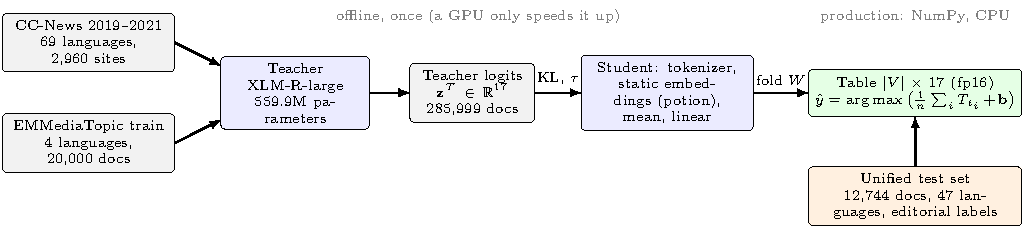
\includegraphics[width=\textwidth]{figures/fig_pipeline.pdf}
\caption{\en{Pipeline} StaticKD. \en{Teacher} melabeli korpus berita tak berlabel satu kali dalam langkah \en{offline}. \en{Student} belajar meniru distribusi \en{teacher}. \en{Head} linear \en{student} kemudian dilipat ke dalam tabel token. Inferensi tereduksi menjadi \en{lookup} dan rata-rata baris tabel. Evaluasi akhir memakai \en{test set} yang labelnya tidak berasal dari \en{teacher}.}
\label{fig:pipeline}
\end{figure*}

\subsection{Formulasi Masalah}
Model memprediksi satu label $y\in\mathcal{Y}$ dari 17 topik IPTC tingkat atas untuk artikel berita $d$ dalam bahasa apa pun. Input berupa judul dan isi artikel yang dipotong hingga 512 kata pertama seperti pada~\cite{kuzman2025llm}. Setiap model kemudian menerapkan batas tokennya sendiri pada input ini (Bagian~\ref{sec:teacher} dan~\ref{sec:student}). \en{Teacher} $f_T$ mengeluarkan logit $\mathbf{z}^T(d)\in\mathbb{R}^{17}$ untuk input tersebut. Studi ini mencari \en{student} $f_S$ yang akurasinya terhadap label independen sedekat mungkin dengan akurasi $f_T$. Inferensi $f_S$ dibatasi pada $O(n)$ penjumlahan untuk $n$ token tanpa perkalian matriks maupun pustaka \en{deep learning}.

\subsection{\en{Teacher} dan Label Distilasi}
\label{sec:teacher}
\en{Teacher} adalah pengklasifikasi IPTC dari~\cite{kuzman2025llm} yang dipublikasikan sebagai \url{classla/multilingual-IPTC-news-topic-classifier}. Pengklasifikasi ini adalah model XLM-RoBERTa-large dengan 24 lapisan, 559.9 juta parameter, dan batas input 512 token XLM-R. \en{Teacher} melabeli seluruh data distilasi dengan biaya satu kali sekitar 1.6 jam GPU dan menghasilkan vektor logit lengkap $\mathbf{z}^{T}(d)\in\mathbb{R}^{17}$ yang disimpan untuk setiap dokumen distilasi.

\subsection{\en{Student} StaticKD}
\label{sec:student}
\en{Student} dibangun di atas model \en{embedding} statis multibahasa potion-multilingual-128M (potion) dari Model2Vec~\cite{tulkens2024model2vec}. Matriks \en{embedding} $E$ \en{student} diinisialisasi dari potion sehingga token dari 101 bahasa berada dalam satu ruang bersama sebelum pelatihan dimulai. Dokumen $d$ ditokenisasi menjadi $t_1,\dots,t_n$ dengan Unigram \en{tokenizer} milik potion yang berisi 500,353 token sehingga setiap token memiliki \en{embedding} hasil prapelatihan. Token khusus tidak dipakai dan token yang tidak dikenal dibuang. Perataan tidak bergantung pada posisi sehingga model tidak memiliki batas panjang bawaan dan panjang dokumen dipotong pada 1,024 token hanya untuk membatasi biaya. Hanya 5.4\% artikel \en{test set} yang melampaui batas ini. \en{Student} menghitung logit dokumen dari rata-rata \en{embedding} token $\mathbf{e}_t\in\mathbb{R}^{256}$:
\begin{equation}
\mathbf{h}(d)=\frac{1}{n}\sum_{i=1}^{n}\mathbf{e}_{t_i},\qquad
\mathbf{z}^{S}(d)=W\,\mathrm{drop}(\mathbf{h}(d))+\mathbf{b},
\label{eq:student}
\end{equation}
dengan $W\in\mathbb{R}^{17\times 256}$ dan \en{dropout} 0.1 pada $\mathbf{h}(d)$ selama pelatihan.

\en{Student} belajar dari logit \en{teacher} yang tersimpan dengan \en{loss}
\begin{equation}
\mathcal{L}_{\mathrm{KD}}=\tau^{2}\,\mathrm{KL}\!\left(p^{T}\,\middle\|\,p^{S}\right),\qquad \tau=1 ,
\label{eq:kd}
\end{equation}
dengan $p^{T}=\mathrm{softmax}(\mathbf{z}^{T}/\tau)$ dan $p^{S}=\mathrm{softmax}(\mathbf{z}^{S}/\tau)$ sebagai distribusi \en{teacher} dan \en{student}. Nilai $\tau=1$ ditetapkan bersama pilihan resep lainnya (Bagian~\ref{sec:roles}) dan hasil untuk nilai lain $\tau\in\{0.5,2,4\}$ dilaporkan pada Bagian~\ref{sec:res-abl}. Parameter $E$, $W$, dan $\mathbf{b}$ dilatih bersama. AdamW ($\eta=3\cdot 10^{-3}$, \en{weight decay} $10^{-4}$) memperbarui $W$ dan $\mathbf{b}$ sedangkan SparseAdam ($\eta=10^{-3}$) memperbarui matriks \en{embedding} $E$ hanya pada baris token yang muncul dalam \en{batch} saat ini. Token yang tidak pernah muncul dalam dokumen pelatihan karena itu tetap memakai \en{embedding} potion. Pelatihan berjalan selama 6 \en{epoch} dengan ukuran \en{batch} 64. \en{Token dropout} menjadi augmentasi yang murah dengan membuang setiap token dalam dokumen pelatihan dengan probabilitas 0.2 pada setiap langkah agar model tidak bergantung pada segelintir kata kunci. Augmentasi ini berbeda dari \en{dropout} 0.1 pada $\mathbf{h}(d)$ dalam Persamaan~\eqref{eq:student}. Validasi internal memakai 3\% data distilasi (8,579 dokumen) untuk menyimpan \en{epoch} dengan \en{agreement} tertinggi terhadap \en{teacher}.

\subsection{\en{Folding}, \en{Ensemble} Tabel, dan Varian Ringkas}
\label{sec:fold}
\en{Head} klasifikasi yang linear memungkinkan \eqref{eq:student} ditulis ulang sebagai
\begin{equation}
W\Big(\frac{1}{n}\sum_{i}\mathbf{e}_{t_i}\Big)+\mathbf{b}=\frac{1}{n}\sum_{i}T_{t_i}+\mathbf{b},
\label{eq:fold}
\end{equation}
dengan tabel $T=EW^{\top}\in\mathbb{R}^{|V|\times 17}$ yang dihitung satu kali setelah pelatihan dalam langkah \en{folding}. Baris $T_t$ pada tabel $T$ memuat 17 skor topik yang disumbangkan token $t$ ke setiap artikel yang mengandungnya. Gambar~\ref{fig:folding} memperlihatkan bahwa matriks $E$ berdimensi 256 hanya diperlukan selama pelatihan sehingga model hasil \en{folding} untuk penerapan hanya terdiri atas $T$ dalam \en{half-precision} (fp16), $\mathbf{b}$, dan \en{tokenizer}. Argumen \en{folding} yang sama berlaku untuk \en{ensemble} karena Persamaan~\eqref{eq:fold} linear terhadap $T$. Perataan logit dari $K$ \en{student} yang dilatih dengan \en{seed} berbeda memberikan hasil yang sama dengan satu \en{student} bertabel $\bar{T}=\frac{1}{K}\sum_k T^{(k)}$ dan berbias $\bar{\mathbf{b}}$.

\begin{figure*}[!t]
\centering
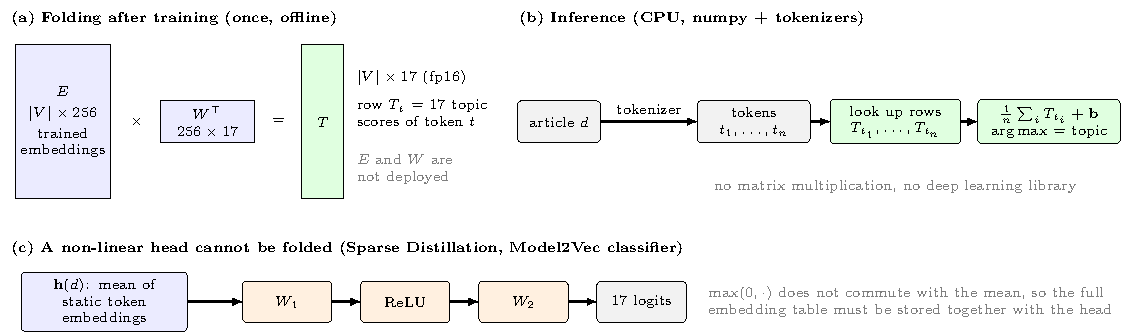
\includegraphics[width=\textwidth]{figures/fig_folding.pdf}
\caption{Mekanisme \en{folding}. (a) \en{Embedding} $E$ dan \en{head} linear $W$ dilipat satu kali setelah pelatihan menjadi tabel $T$. (b) Inferensi hanya memerlukan tokenisasi, \en{lookup} baris $T$, dan perataan. (c) \en{Head} nonlinear mencegah \en{folding} sehingga $E$ harus tetap disimpan.}
\label{fig:folding}
\end{figure*}

Model StaticKD akhir merata-ratakan tabel dari tiga \en{student} ($K=3$) dan memiliki 8.5 juta parameter. Berkas model ini berukuran 34~MB dan tabel hasil perataan menyumbang 16~MB dari ukuran tersebut. Sebagian besar \en{random-access memory} (RAM) yang dipakai model ini saat inferensi diisi struktur internal Unigram \en{tokenizer}. Varian ringkas memperkecil struktur tersebut dengan menghapus potongan token yang muncul kurang dari 10 kali dalam data distilasi tetapi tetap menyimpan karakter tunggal. Kosakata varian ini berisi 335,441 token dan berkasnya berukuran 23~MB.

\section{Data dan \en{Test Set}}
\label{sec:data}
\subsection{Set Data dan Perannya}
\label{sec:roles}
Tabel~\ref{tab:datasets} menunjukkan bahwa \en{development set} dan validasi internal yang dipakai untuk memilih pengaturan model terpisah dari \en{test set} terpadu. \en{Development set} adalah set data berlabel yang dipakai untuk memilih pengaturan model sebelum pengukuran akhir sehingga \en{test set} tidak ikut memengaruhi pilihan tersebut. \en{Development set} studi ini adalah \en{split} pengembangan EMMediaTopic (Bagian~\ref{sec:distdata}). Pengaturan parameter dan pilihan resep StaticKD ditentukan sebelum \en{test set} dibangun. \en{Development set} juga dipakai untuk menguji empat komponen tambahan: fitur bigram, \en{pooling} berbobot idf, pembobotan dokumen menurut keyakinan \en{teacher}, dan \en{loss} tambahan pada label GPT-4o. Keempatnya tidak dimasukkan ke resep karena tidak mengubah skor \en{development set} secara signifikan.

\begin{table}[!t]
\caption{Set Data Studi dan Perannya}
\label{tab:datasets}
\centering
\footnotesize
\setlength{\tabcolsep}{3pt}
\resizebox{\columnwidth}{!}{%
\begin{tabular}{@{}lrrll@{}}
\toprule
Set & Dok. & Bahasa & Label & Dipakai untuk \\
\midrule
Data distilasi & 285,999 & 69 & teacher & melatih student \\
\quad validasi internal & 8,579 & -- & teacher & memilih epoch \\
Development (EMMediaTopic) & 1,000 & 4 & GPT-4o & memilih resep \\
CC-News held-out & 12,554 & 63 & teacher & agreement, situs di luar distilasi \\
Test set terpadu & 12,744 & 47 & manusia, editorial & semua hasil akurasi \\
Sampel rubrik bahasa Inggris & 754 & 1 & JSON-LD & hanya validitas label \\
\bottomrule
\end{tabular}}
\end{table}

\subsection{Data Distilasi dan \en{Development Set}}
\label{sec:distdata}
\en{Development set} dan sebagian data distilasi bersumber dari EMMediaTopic 1.0~\cite{emmediatopic2025,kuzman2025llm}. EMMediaTopic berisi artikel berlabel GPT-4o dalam empat bahasa (Katalan, Yunani, Kroasia, dan Slovenia). Sebanyak 21,000 artikel beranotasi diambil dan dibagi menjadi \en{split} pelatihan berisi 20,000 artikel dan \en{split} pengembangan berisi 1,000 artikel. Kuzman dan Ljube\v{s}i\'c melatih \en{teacher} pada \en{split} pelatihan dan menyetel \en{hyperparameter} \en{teacher} pada \en{split} pengembangan~\cite{kuzman2025llm}. \en{Split} pelatihan juga menjadi bagian dari data distilasi untuk \en{student}. Baik \en{teacher} maupun \en{student} tidak pernah dilatih pada \en{split} pengembangan.

Sebagian besar data distilasi berasal dari \en{dataset} multibahasa CC-News 2019--2021~\cite{cloversearch_ccnews} yang dibangun dari arsip berita Common Crawl. CC-News 2019--2021 diolah dengan langkah-langkah berikut.
\begin{enumerate}
  \item Periksa bahasa dengan model identifikasi bahasa fastText~\cite{joulin2017bag} dan pertahankan hanya dokumen yang bahasa metadatanya sesuai dengan bahasa hasil identifikasi.
  \item Pertahankan dokumen yang judul dan isinya mencapai total 75 kata dan potong teks menjadi 512 kata. Dokumen dalam bahasa Jepang, Mandarin, Thai, dan Burma memakai batas 200 dan 2,000 karakter sebagai gantinya.
  \item Sisihkan semua dokumen dari sebagian situs ke dalam \en{held-out set} yang tidak dipakai untuk pelatihan dan memuat paling banyak 20\% dari tiap bahasa.
  \item Batasi jumlah dokumen pelatihan per situs untuk menghindari bias dari konten serupa dalam satu situs.
\end{enumerate}
Data distilasi akhir berisi 285,999 dokumen dalam 69 bahasa dari 2,960 situs dengan median panjang dokumen 269 kata dan paling banyak 400 dokumen per situs. Data ini terdiri atas versi dasar berisi sekitar 130 ribu dokumen dengan paling banyak 150 dokumen per situs dan 156,157 dokumen tambahan dari situs pelatihan saja (paling banyak 5,000 per bahasa). Versi dasar juga dipakai sebagai varian ablasi (Bagian~\ref{sec:design}).

\en{Held-out set} berisi 12,554 dokumen dalam 63 bahasa dari 217 situs yang tidak pernah muncul dalam data distilasi. Set ini hanya dapat mengukur \en{agreement} dengan \en{teacher} karena tidak memiliki label kategori independen.

\subsection{Pembentukan \en{Test Set} Terpadu}
\label{sec:testset}
Sumber terbesar \en{test set} terpadu adalah \en{dataset} CC-NEWS 2024--2026~\cite{commoncrawl2026ccnews} yang disampel sebagai satu berkas arsip (WARC) per bulan dari Januari 2024 hingga Agustus 2026 (32 berkas). Setiap halaman artikel memuat metadata terstruktur schema.org~\cite{guha2016schema} dalam format JSON-LD yang menyediakan rubrik artikel dan metadata lain dalam kolom seperti \texttt{articleSection}, \texttt{BreadcrumbList}, \texttt{inLanguage}, \texttt{datePublished}, \texttt{isAccessibleForFree}, dan \texttt{articleBody}. Teks diambil dari \texttt{articleBody} hanya bila kolom itu berisi paling sedikit 30 kata. Teks artikel lain diekstrak dari konten HTML dengan pustaka Trafilatura~\cite{barbaresi2021trafilatura}.

Artikel \en{test set} lainnya berasal dari kelima \en{dataset} publik pada Bagian~\ref{sec:rw-iptc}. Artikel L3Cube-IndicNews diambil dari \en{split} LDC yang berisi dokumen panjang. Kategori penerbit pada \en{dataset} ini dan rubrik JSON-LD sama-sama termasuk label editorial.

Label editorial tidak mengikuti standar IPTC sehingga nama rubrik harus diterjemahkan ke pohon IPTC Media Topic resmi (1,085 \en{node} aktif). Nama rubrik dinormalisasi untuk huruf besar-kecil dan diakritik lalu dipetakan secara konservatif oleh LLM (Claude Opus 5.5). LLM hanya membaca nama rubrik tanpa teks artikel dan memetakan sebuah nama hanya jika pokok bahasan yang dinyatakan nama itu berada di bawah satu topik tingkat atas dalam pohon IPTC. Pemeriksaan otomatis memastikan bahwa setiap \en{node} tujuan ada dalam pohon IPTC, masih aktif, dan berada di bawah topik tingkat atas yang dimaksud. Tabel pemetaan yang disusun LLM kemudian dievaluasi dan dikoreksi secara manual oleh peninjau manusia. Tabel akhir menghubungkan 814 nama rubrik ke 79 \en{node} IPTC. Artikel yang rubrik-rubriknya dalam kolom \texttt{articleSection} dan \texttt{BreadcrumbList} terpetakan ke label berbeda ditolak agar setiap artikel memiliki satu label.

Filter kualitas dan kebocoran diterapkan secara berurutan.
\begin{enumerate}
  \item Situs belum muncul dalam data distilasi maupun dalam \en{held-out set} (hanya CC-NEWS).
  \item Tanggal terbit pada atau setelah 1 Januari 2024 (hanya CC-NEWS).
  \item Teks artikel lengkap dan tidak berupa cuplikan (\en{teaser}).
  \item Bahasa yang dinyatakan sesuai dengan identifikasi bahasa fastText bila fastText mendukung bahasa tersebut.
  \item Paling sedikit 75 kata.
  \item Deduplikasi \en{uniform resource locator} (URL), teks identik, dan teks hampir duplikat (MinHash~\cite{broder1997resemblance}, Jaccard $\ge 0.7$~\cite{lee2022dedup}) di seluruh sumber.
  \item Kontaminasi: artikel dibuang bila $\ge 30\%$ dari 8-gram katanya muncul dalam salah satu dari sekitar 300 ribu dokumen pelatihan atau evaluasi.
\end{enumerate}

Artikel yang lolos semua filter disampel dengan paling banyak 50 artikel untuk setiap pasangan bahasa dan label dengan mendahulukan sumber berlabel manusia. \en{Test set} akhir berisi 12,744 artikel dalam 47 bahasa dari 1,227 situs atau sumber dengan median panjang artikel 313 kata. Seluruh 17 label muncul dalam \en{test set} ini meskipun artikel suatu bahasa mencakup median 7 dari 17 label. \emph{Asal label} artikel adalah anotasi manusia untuk 4,094 artikel (32.1\%), kategori penerbit untuk 2,600 artikel (20.4\%), dan rubrik JSON-LD untuk 6,050 artikel (47.5\%). Tabel~\ref{tab:testset} menunjukkan bahwa keragaman penerbit terutama berasal dari CC-NEWS yang mencakup 1,092 situs dalam 29 bahasa.

\begin{figure*}[!t]
\centering
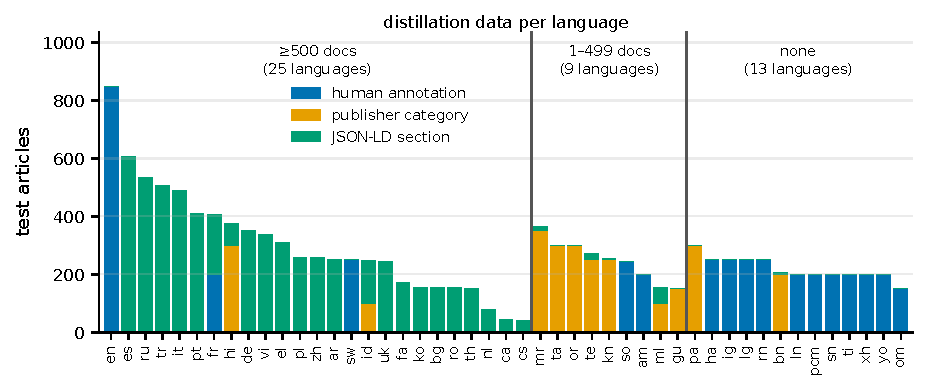
\includegraphics[width=\textwidth]{figures/fig_testset_composition.pdf}
\caption{Jumlah artikel \en{test set} terpadu per bahasa menurut asal label. Bahasa dikelompokkan menurut jumlah dokumen distilasinya.}
\label{fig:testset}
\end{figure*}

Jumlah data distilasi berbeda antarbahasa \en{test set} dan dipakai untuk analisis subkelompok (Bagian~\ref{sec:protocol}). Data distilasi tidak tersedia untuk 13 bahasa sedangkan 9 bahasa lain memiliki kurang dari 500 dokumen distilasi dan 25 bahasa sisanya memiliki paling sedikit 500. Gambar~\ref{fig:testset} memperlihatkan bahwa label bahasa tanpa data distilasi atau dengan sedikit data distilasi hampir seluruhnya berasal dari anotasi manusia atau kategori penerbit sedangkan rubrik JSON-LD terutama mencakup bahasa dengan paling sedikit 500 dokumen distilasi.

\begin{table}[!t]
\caption{Komposisi \en{Test Set} Terpadu menurut Sumber}
\label{tab:testset}
\centering
\footnotesize
\setlength{\tabcolsep}{3pt}
\resizebox{\columnwidth}{!}{%
\begin{tabular}{@{}llrrr@{}}
\toprule
Sumber & Asal label & Artikel & Bahasa & Situs/sumber \\
\midrule
CC-NEWS 2024--2026 & rubrik JSON-LD & 6,050 & 29 & 1,092 \\
MasakhaNEWS~\cite{adelani2023masakhanews} & anotasi manusia & 3,339 & 16 & 6 \\
L3Cube-IndicNews~\cite{mirashi2023indicnews} & kategori penerbit & 2,361 & 10 & 1 \\
MN-DS~\cite{petukhova2023mnds} & anotasi manusia & 755 & 1 & 127 \\
Bangla news~\cite{hossain2025banglanews} & kategori penerbit & 139 & 1 & 1 \\
IndoNews & kategori penerbit & 100 & 1 & 1 \\
\midrule
Total & & 12,744 & 47 & 1,227 \\
\bottomrule
\end{tabular}}
\par\vspace{2pt}{\footnotesize Satu situs (jpost.com) muncul di CC-NEWS dan di MN-DS sehingga total situs satu lebih kecil daripada jumlah kolom.\par}
\end{table}

\subsection{Pemeriksaan Validitas Label}
\label{sec:validity-design}
Dua pertiga label pada \en{test set} adalah label rubrik dan kategori yang mencatat keputusan redaksi dan bukan anotasi yang mengikuti pedoman pelabelan. Pemeriksaan validitas label menguji apakah label semacam itu berperilaku seperti label manusia dalam bahasa yang sama (Bagian~\ref{sec:res-validity}). \en{Teacher} yang sama hanya menjadi acuan tetap bagi kedua jenis label sehingga label rubrik dengan \en{noise} yang jauh lebih banyak akan membuat \en{teacher} lebih jarang cocok dengan label rubrik daripada dengan label manusia. Kecocokan ini diukur dengan akurasi dan macro-F1 \en{teacher} pada tiap jenis label, uji Wilcoxon \en{signed-rank} atas akurasi per label, dan korelasi Spearman antara peringkat kesulitan label pada kedua jenis label. Analisis per kategori sumber juga memeriksa pemetaan dengan membandingkan prediksi \en{teacher} dan label hasil pemetaan pada tiap kategori sumber dalam bahasa yang tercakup dalam prapelatihan XLM-R.

Perbandingan antarjenis label memerlukan label rubrik dan label manusia dalam bahasa yang sama. \en{Test set} sendiri menyediakan label rubrik dan label manusia MasakhaNEWS dalam bahasa Prancis. Bagian bahasa Inggris dari \en{test set} hanya berisi label manusia karena penyampelan mendahulukan sumber berlabel manusia (Bagian~\ref{sec:testset}). Perbandingan di dalam bahasa Inggris harus memakai sampel artikel yang tidak termasuk dalam \en{test set}. Sampel ini berisi 754 artikel CC-NEWS berbahasa Inggris dari 306 situs dengan label rubrik JSON-LD dan paling banyak 50 artikel per label.

\section{Pengaturan Eksperimen}
\label{sec:setup}
\subsection{\en{Baseline}}
\label{sec:baselines}
Semua \en{baseline} bertanda + KD belajar dari data distilasi yang sama (285,999 dokumen) dan dari \en{teacher} yang sama. Tabel~\ref{tab:baselines} menunjukkan bahwa hanya kedua \en{baseline} \en{transformer} yang belajar dari distribusi penuh \en{teacher}. Tiga \en{baseline} ringan dilatih pada label teratas \en{teacher} karena prosedur pelatihan standarnya menerima label kelas tetapi tidak menerima distribusi probabilitas. Ketiga \en{baseline} ringan itu adalah fastText + KD~\cite{joulin2017bag}, \en{term frequency--inverse document frequency} (TF-IDF) + \en{support vector machine} (SVM) + KD, dan pengklasifikasi Model2Vec + KD~\cite{tulkens2024model2vec}. TF-IDF + SVM + KD mengadaptasi \en{baseline} nonneural dari Kuzman dan Ljube\v{s}i\'c ke label \en{teacher}. Pengklasifikasi Model2Vec + KD menerapkan \en{fine-tuning} pada \en{embedding} potion yang juga menjadi titik awal StaticKD serta mempelajari bobot untuk tiap token. Dua model fastText lain dilatih hanya pada label GPT-4o dari \en{split} pelatihan EMMediaTopic sebagai acuan tanpa KD yang memakai data berlabel yang sama dengan \en{teacher}~\cite{kuzman2025llm}.

MiniLM-L6 + KD dan DistilmBERT + KD adalah \en{baseline} \en{transformer} yang dilatih dengan \en{loss}~\eqref{eq:kd} pada distribusi penuh \en{teacher}. MiniLM-L6 + KD memakai mMiniLMv2-L6-H384 yang didistilasi dari XLM-R-large~\cite{wang2021minilmv2} sedangkan DistilmBERT + KD memakai \texttt{distilbert-base-multilingual-cased}~\cite{sanh2019distilbert}. Batas 256 token memotong 91.1\% artikel \en{test} menjadi sekitar 142 kata untuk MiniLM-L6 dan 93.2\% menjadi sekitar 116 kata untuk DistilmBERT. Pemeriksaan sensitivitas terhadap batas ini melatih ulang kedua model dengan 512 token (Bagian~\ref{sec:res-acc}).

Sparse Distillation~\cite{ye2022sparse} adalah metode terdahulu yang paling dekat dengan StaticKD tetapi tidak dijalankan sebagai \en{baseline} tersendiri (Bagian~\ref{sec:limitations}). Sebagian dari metode tersebut tetap tercakup dalam dua eksperimen lain. \en{Baseline} fastText + KD melatih model \en{bag-of-n-grams} dengan perataan dan \en{head} linear pada label \en{teacher} yang sama. Ablasi inisialisasi acak (Bagian~\ref{sec:design}) melatih tabel \en{embedding} dari awal seperti Sparse Distillation.

\begin{table*}[!t]
\caption{\en{Baseline} dan Cara Pelatihannya}
\label{tab:baselines}
\centering
\footnotesize
\setlength{\tabcolsep}{4pt}
\resizebox{\textwidth}{!}{%
\begin{tabular}{@{}llll@{}}
\toprule
Model & Representasi saat inferensi & Target pelatihan & Penyetelan \\
\midrule
fastText + KD, kata & rata-rata vektor kata dan n-gram karakter, head linear & label teratas teacher & grid search pada development set \\
fastText + KD, subword & rata-rata vektor subword XLM-R, head linear & label teratas teacher & grid search pada development set \\
fastText + KD, subword, terkuantisasi & varian subword dalam format \texttt{.ftz} & label teratas teacher & dari varian subword \\
TF-IDF + SVM + KD & TF-IDF atas subword XLM-R, SVM linear & label teratas teacher & grid search pada development set \\
Pengklasifikasi Model2Vec + KD & embedding potion hasil fine-tuning dengan bobot per token, lapisan tersembunyi 512 unit & label teratas teacher & pengaturan bawaan pustaka \\
MiniLM-L6 + KD & transformer 6 lapisan, input 256 token & distribusi penuh teacher & $\tau\in\{1,2\}$ pada development set \\
DistilmBERT + KD & transformer 6 lapisan, input 256 token & distribusi penuh teacher & $\tau=1$ \\
fastText, label GPT-4o (kata, subword) & seperti fastText + KD & label GPT-4o EMMediaTopic & pengaturan tetap \\
\bottomrule
\end{tabular}}
\end{table*}

\subsection{Protokol Evaluasi dan Uji Statistik}
\label{sec:protocol}
Tabel~\ref{tab:protocol} menempatkan macro-F1 sebagai metrik utama karena distribusi label tidak seimbang. Metrik ini adalah rata-rata F1 tak tertimbang atas label yang ada dalam referensi sesuai protokol evaluasi~\cite{kuzman2025llm}. Macro-F1 per bahasa dirata-ratakan atas bahasa agar bahasa besar tidak mendominasi. Kalibrasi diukur dengan \en{expected calibration error} (ECE)~\cite{guo2017calibration} karena mode \en{cascade} pada Bagian~\ref{sec:effprotocol} mengarahkan artikel menurut tingkat keyakinan StaticKD.

Interval kepercayaan dan uji berpasangan memakai \en{bootstrap} dengan unit \en{resampling} yang berbeda pada kedua set evaluasi. \en{Development set} di-\en{resample} per dokumen sedangkan \en{test set} memakai \en{site-cluster bootstrap}~\cite{field2007bootstrapping} yang menarik situs secara utuh sebagai unit \en{resampling} agar artikel yang berkaitan dari satu situs tidak membuat interval kepercayaan terlalu sempit. Artikel tanpa URL dikelompokkan menurut \en{dataset} sumber.

Klaster pada \en{test set} tidak seimbang sehingga dua pemeriksaan tambahan menguji ketahanan perbandingan model. Dua klaster terbesar dari 1,227 klaster (bbc.com dan L3Cube-IndicNews) memuat 37.3\% artikel dan jumlah efektif klaster $1/\sum_c q_c^{2}$ dengan $q_c$ sebagai proporsi klaster $c$ hanya 13.8. Pemeriksaan \en{leave-one-source-out} menghitung ulang macro-F1 \en{teacher} dan StaticKD beserta ketujuh \en{baseline} + KD dengan membuang tiap sumber dari enam sumber \en{test set} satu per satu. Pemeriksaan lain mengulang perbandingan model pada \en{subset} dengan paling banyak lima artikel per situs dan pasangan bahasa--label.

Perbedaan yang tidak signifikan pada uji berpasangan tidak menunjukkan bahwa dua model setara sehingga klaim kesetaraan bertumpu pada \en{two one-sided tests} (TOST) atas distribusi \en{bootstrap} yang sama. Margin 0.01 macro-F1 diperlakukan sebagai perbedaan yang dapat diabaikan untuk penyaringan topik. Koreksi Holm diterapkan terpisah pada \en{development set} dan \en{test set} atas semua perbandingan StaticKD dengan model lain pada Tabel~\ref{tab:sig}.

Perbandingan tiap varian ablasi dengan resep akhir memakai \en{bootstrap} berpasangan yang sama. Setiap \en{resample} menilai semua \en{seed} varian dan resep akhir pada artikel yang sama dan menghasilkan selisih antara kedua rata-rata \en{seed} sebagai besaran yang diuji. Skor \en{ensemble} berisi $K$ \en{student} adalah rata-rata skor atas semua kombinasi $K$ dari sepuluh \en{seed} resep akhir. Koreksi Holm untuk perbandingan ini mencakup 10 varian pada Bagian~\ref{sec:design} dan keempat komponen tambahan dari Bagian~\ref{sec:roles} yang masing-masing dijalankan dengan tiga \en{seed}.

Analisis per bahasa memakai dua besaran. \emph{Selisih akurasi} adalah akurasi StaticKD dikurangi akurasi \en{teacher}. \emph{Cakupan token} suatu bahasa adalah proporsi dari semua kemunculan token dalam artikel \en{test} bahasa tersebut yang tokennya muncul paling sedikit 10 kali dalam data distilasi. Ambang ini dipakai karena pelatihan jarang memperbarui \en{embedding} token yang lebih jarang muncul (Bagian~\ref{sec:student}).

Analisis subkelompok membagi hasil menurut bahasa, aksara, wilayah, label, asal label, keragaman situs, jumlah data distilasi per bahasa, dan cakupan prapelatihan \en{teacher}. Keragaman situs suatu bahasa diukur dengan jumlah efektif situs $1/\sum_s q_s^{2}$ dengan $q_s$ sebagai proporsi artikel bahasa itu yang berasal dari situs $s$. Cakupan prapelatihan menyatakan apakah suatu bahasa termasuk dalam 100 bahasa yang dipakai untuk prapelatihan XLM-R~\cite{conneau2020xlmr}.

Tujuh uji memeriksa apakah sifat suatu bahasa menjelaskan kinerja StaticKD pada bahasa itu dengan nilai $p$ yang dikoreksi Holm bersama-sama. Empat uji memeriksa kemiripan StaticKD dengan \en{teacher} pada 53 bahasa dengan paling sedikit 20 dokumen \en{held-out}. Tiga korelasi Spearman di antaranya mengaitkan \en{agreement} \en{held-out} dengan log jumlah data distilasi, jumlah situs pelatihan, dan tingkat keyakinan \en{teacher} sedangkan uji Kruskal--Wallis membandingkan \en{agreement} antaraksara. Tiga uji lain memeriksa ketertinggalan StaticKD dari \en{teacher} pada \en{test set} melalui korelasi Spearman antara selisih akurasi dan log jumlah data distilasi, antara akurasi StaticKD dan cakupan token, serta antara selisih akurasi dan cakupan token.

Analisis tabel token mengukur \emph{spesifisitas} sebuah token sebagai selisih terbesar antara satu entri pada baris tabelnya dan rata-rata 16 entri lainnya. Uji pemangkasan hanya mempertahankan 10\% token paling spesifik dari tiap artikel dan membandingkan hasilnya dengan hasil dari 10\% token acak untuk mengukur seberapa banyak sinyal topik dibawa token yang paling spesifik.

\begin{table}[!t]
\caption{Ringkasan Protokol Evaluasi dan Uji Statistik}
\label{tab:protocol}
\centering
\footnotesize
\setlength{\tabcolsep}{3pt}
\begin{tabular}{@{}p{0.30\columnwidth}p{0.66\columnwidth}@{}}
\toprule
Pertanyaan & Metrik atau uji \\
\midrule
Akurasi terhadap label independen & macro-F1 (utama), akurasi, dan macro-F1 per bahasa \\
Kemiripan dengan teacher & agreement pada held-out set \\
Kalibrasi & ECE dengan 15 bin \\
Ketidakpastian skor & interval kepercayaan 95\% dari bootstrap persentil dengan 1,000 resample \\
Beda dua model & bootstrap berpasangan dengan 2,000 resample untuk $\Delta$macro-F1~\cite{koehn2004significance}, McNemar eksak untuk akurasi~\cite{mcnemar1947}, dan koreksi Holm~\cite{holm1979} \\
Kesetaraan dua model & TOST~\cite{schuirmann1987tost} dengan interval 90\% dalam $\pm$0.01 \\
Konsistensi antarbahasa & Wilcoxon signed-rank pada macro-F1 dan akurasi per bahasa~\cite{dror2018hitchhiker} \\
Efek komponen resep & ablasi dengan lima seed per varian dan sepuluh seed untuk resep akhir \\
Sifat bahasa & enam korelasi Spearman dan satu uji Kruskal--Wallis dengan koreksi Holm bersama \\
Ketahanan terhadap klaster & leave-one-source-out dan subset dengan paling banyak lima artikel per situs dan pasangan bahasa--label \\
\bottomrule
\end{tabular}
\end{table}

\subsection{Protokol Efisiensi}
\label{sec:effprotocol}
Tabel~\ref{tab:effsetup} menunjukkan bahwa semua model diukur dengan pengaturan yang sama sehingga rasio kecepatan antarmodel dapat dibandingkan. CPU laptop tersebut bersifat hibrida dan memiliki 6 \en{performance core} (P-core), 8 \en{efficiency core} (E-core) yang lebih lambat, dan 2 E-core berdaya rendah. Sistem operasi memindahkan \en{thread} yang tidak dipatok ke \en{core} yang lambat sehingga setiap proses dipatok ke P-core fisik dan pengaturannya menyerupai server kecil dengan \en{core} yang seragam. \en{Throughput} satu \en{core} setiap model menyimpang paling banyak 7\% dari median tiga sesi pengukuran. Profil satu \en{thread} terpisah memecah waktu prediksi StaticKD menjadi waktu tokenisasi dan waktu perataan tabel pada 1,280 artikel untuk mengetahui langkah yang membatasi kecepatannya.

Kedua \en{baseline} \en{transformer} diekspor ke format Open Neural Network Exchange (ONNX) dalam fp32 untuk \en{benchmark} CPU. \en{Teacher} juga diekspor ke ONNX dengan kuantisasi dinamis ke bilangan bulat 8-bit (int8). Versi ONNX int8 ini adalah konfigurasi \en{teacher} tercepat pada CPU.

\begin{table}[!t]
\caption{Pengaturan \en{Benchmark} CPU}
\label{tab:effsetup}
\centering
\footnotesize
\setlength{\tabcolsep}{3pt}
\begin{tabular}{@{}p{0.22\columnwidth}p{0.74\columnwidth}@{}}
\toprule
Aspek & Pengaturan \\
\midrule
Mesin & laptop Intel Core Ultra~7 155H, RAM 32~GB, Windows~11, GPU dinonaktifkan \\
Proses & proses baru per model, jumlah thread dipatok di setiap pustaka, satu atau empat P-core fisik \\
Sampel & sampel teks acak yang sama dari test set terpadu \\
Latensi & median (p50) dan persentil ke-95 (p95) dengan satu artikel per panggilan (skenario streaming); 100 dokumen untuk teacher dan transformer, 500 dokumen untuk model ringan \\
Throughput & batch 64 (8 untuk transformer); 96 dokumen untuk teacher dan transformer, 3,000 dokumen untuk model ringan \\
RAM model & kenaikan resident set size setelah model dimuat \\
Pengulangan & tiga sesi pada mesin yang menganggur, median dilaporkan \\
\bottomrule
\end{tabular}
\end{table}

Perbandingan kecepatan tidak menguntungkan StaticKD karena StaticKD membaca input yang lebih panjang. StaticKD membaca hingga 1,024 token per artikel sedangkan \en{teacher} berhenti pada 512 token XLM-R. Batas \en{teacher} ini terlampaui pada 60.7\% artikel \en{test set} dan pada artikel tersebut \en{teacher} membaca sekitar 287 dari 438 kata (median).

Mode \en{cascade} menggabungkan StaticKD dan \en{teacher} untuk pekerjaan yang memerlukan akurasi setingkat \en{teacher}. Mode ini membiarkan StaticKD memutuskan artikel yang probabilitas teratasnya paling sedikit sebesar ambang $\theta$. Artikel sisanya diteruskan ke \en{teacher} ONNX int8. Misalkan $s$ adalah proporsi artikel yang diputuskan oleh StaticKD serta $r_S$ dan $r_T$ adalah \en{throughput} satu \en{core} StaticKD dan \en{teacher}. \en{Throughput} efektif \en{cascade} adalah $1/(1/r_S+(1-s)/r_T)$.

\subsection{Rancangan Ablasi}
\label{sec:design}
Tiap varian ablasi mengubah satu faktor dari resep akhir. Satu varian mengganti \en{soft label} dengan \en{hard label} dan dua varian mengurangi data pelatihan menjadi EMMediaTopic saja (4 bahasa, 10 \en{epoch}) atau menjadi 130 ribu dokumen tanpa data tambahan CC-News 2019--2021. Varian lain membekukan \en{embedding} atau mengambil \en{embedding} acak dengan simpangan baku yang sama dengan potion. Varian sisanya dilatih tanpa \en{token dropout}, memakai \en{head} MLP 512 unit, atau menetapkan $\tau\in\{0.5,\,2,\,4\}$. Tabel~\ref{tab:ablation} memuat resep akhir dan seluruh varian ini.

\subsection{Detail Implementasi}
\label{sec:impl}
Satu \en{run} StaticKD rata-rata memakan waktu 5.2 menit pada NVIDIA RTX~4050 Laptop GPU. Implementasi memakai Python~3.12, NumPy~2.5, PyTorch~2.6, transformers~5.17, \texttt{tokenizers}~0.23, ONNX Runtime~1.30, scikit-learn~1.9, dan fastText~0.9.2.

\section{Hasil}
\label{sec:results}
\subsection{Validitas Label Editorial}
\label{sec:res-validity}
Kecocokan \en{teacher} dengan kedua jenis label menunjukkan bahwa label rubrik bahasa Inggris tidak mengandung \en{noise} lebih banyak daripada label manusia. \en{Teacher} mencapai akurasi 0.646 pada 754 artikel bahasa Inggris berlabel rubrik (macro-F1 0.617) dan 0.559 pada label manusia bahasa Inggris dari MN-DS dan MasakhaNEWS (macro-F1 0.565). \en{Teacher} lebih akurat pada label rubrik untuk 12 dari 17 label (Wilcoxon $p=0.033$). Peringkat kesulitan label juga berkorelasi antara kedua jenis label ($\rho=0.63$, $p=0.007$) dan label sulit yang sama pada keduanya adalah \emph{society}, \emph{human interest}, dan \emph{religion}. Data bahasa Prancis dalam \en{test set} juga memuat kedua jenis label dan menunjukkan arah yang sama dengan akurasi \en{teacher} 0.716 pada 208 artikel berlabel rubrik dibandingkan 0.500 pada 200 artikel MasakhaNEWS berlabel manusia.

Kecocokan per kategori antara \en{teacher} dan label hasil pemetaan terendah pada kategori sumber yang lebih luas daripada target IPTC dan pada label dengan batas yang tidak jelas. Median kecocokan per kategori lebih tinggi untuk L3Cube (0.81) dan rubrik CC-NEWS (0.87) daripada untuk MasakhaNEWS (0.46) dan MN-DS (0.50). Kategori \emph{politics} pada MasakhaNEWS hanya memiliki 45\% artikel yang diprediksi sebagai \emph{politics} dengan \emph{conflict} (29\%) sebagai alternatif utama. Label \emph{society} pada MN-DS adalah contoh label dengan batas yang tidak jelas.

\subsection{Akurasi Semua Model}
\label{sec:res-acc}
\begin{table*}[!t]
\caption{Hasil Utama. Macro-F1 [95\% CI] dan Akurasi pada \en{Development Set} (EMMediaTopic Dev, Label GPT-4o), \en{Agreement} dengan \en{Teacher} pada CC-News \en{Held-Out}, dan Hasil pada \en{Test Set} Terpadu (47 Bahasa, Label Independen). CI \en{Test} dari \en{Site-Cluster Bootstrap}}
\label{tab:main}
\centering
\scriptsize
\setlength{\tabcolsep}{3.5pt}
\begin{tabular}{@{}lccccccc@{}}
\toprule
 & \multicolumn{2}{c}{dev (4 bahasa)} & held-out & \multicolumn{4}{c}{test terpadu (47 bahasa)} \\
\cmidrule(lr){2-3}\cmidrule(lr){4-4}\cmidrule(lr){5-8}
Model & Macro-F1 [95\% CI] & Akurasi & Agreement & Macro-F1 [95\% CI] & Akurasi & Macro-F1/bahasa & \% teacher \\
\midrule
Teacher XLM-R-large & 0.822 [0.779--0.851] & 0.859 & -- & 0.598 [0.546--0.643] & 0.700 & 0.705 & 100.0\% \\
Teacher XLM-R-large, ONNX int8 & 0.823 [0.781--0.852] & 0.858 & -- & 0.600 [0.547--0.646] & 0.699 & 0.702 & 100.3\% \\
\midrule
DistilmBERT + KD & 0.753 [0.710--0.785] & 0.801 & 0.799 & 0.534 [0.481--0.618] & 0.623 & 0.602 & 89.4\% \\
MiniLM-L6 + KD & 0.785 [0.737--0.815] & 0.820 & 0.825 & 0.566 [0.511--0.624] & 0.667 & 0.661 & 94.6\% \\
\midrule
\textbf{StaticKD (usulan)} & \textbf{0.761 [0.717--0.792]} & 0.800 & 0.811 & \textbf{0.545 [0.490--0.605]} & 0.641 & 0.622 & 91.1\% \\
StaticKD ringkas & 0.754 [0.710--0.786] & 0.797 & 0.802 & 0.484 [0.421--0.597] & 0.544 & 0.507 & 81.0\% \\
\midrule
fastText + KD, subword, terkuantisasi & 0.729 [0.688--0.760] & 0.768 & 0.740 & 0.439 [0.370--0.561] & 0.515 & 0.465 & 73.4\% \\
fastText + KD, subword & 0.737 [0.701--0.765] & 0.772 & 0.754 & 0.447 [0.385--0.566] & 0.527 & 0.480 & 74.7\% \\
fastText + KD, kata & 0.750 [0.713--0.779] & 0.791 & 0.758 & 0.445 [0.380--0.563] & 0.515 & 0.474 & 74.5\% \\
TF-IDF + SVM + KD & 0.755 [0.719--0.786] & 0.798 & 0.776 & 0.486 [0.431--0.585] & 0.567 & 0.522 & 81.3\% \\
Pengklasifikasi Model2Vec + KD & 0.744 [0.701--0.772] & 0.780 & 0.805 & 0.547 [0.495--0.599] & 0.642 & 0.619 & 91.5\% \\
\midrule
fastText, label GPT-4o, subword & 0.665 [0.613--0.700] & 0.729 & 0.260 & 0.086 [0.069--0.119] & 0.150 & 0.118 & 14.4\% \\
fastText, label GPT-4o, kata & 0.651 [0.601--0.693] & 0.738 & 0.307 & 0.106 [0.085--0.150] & 0.181 & 0.142 & 17.7\% \\
\bottomrule
\end{tabular}
\end{table*}
Tabel~\ref{tab:main} menunjukkan bahwa StaticKD mempertahankan 91.1\% macro-F1 \en{teacher} pada \en{test set} terpadu dan 92.6\% pada \en{development set}. Macro-F1 \en{test} StaticKD adalah 0.545 [0.490--0.605] dan macro-F1 \en{test} \en{teacher} 0.598 [0.546--0.643]. Skor \en{test} kedua model lebih rendah daripada skor \en{development set} (0.761 dan 0.822) karena sebagian besar \en{test set} berada di luar bahasa, sumber, dan periode data pelatihan \en{teacher}. Prediksi StaticKD sama dengan prediksi \en{teacher} pada 81.1\% dokumen \en{held-out} dalam 63 bahasa.

Macro-F1 \en{test} StaticKD berada di antara skor kedua \en{transformer} hasil distilasi dan di atas skor fastText + KD serta TF-IDF + SVM + KD. Skor MiniLM-L6 (0.566) lebih tinggi daripada StaticKD sedangkan skor DistilmBERT (0.534) sedikit lebih rendah. Pengklasifikasi Model2Vec mencapai 0.547 atau hampir sama dengan StaticKD. Model fastText yang dilatih hanya pada label GPT-4o dari empat bahasa memperlihatkan akibat ketiadaan label \en{teacher} untuk bahasa lain (dua baris terakhir pada Tabel~\ref{tab:main}). Skor model ini mencapai 0.665 pada \en{development set} tetapi hanya 0.086 pada \en{test set}.

\begin{table*}[!t]
\caption{Uji Berpasangan StaticKD terhadap Model Lain pada \en{Test Set} Terpadu. $\Delta$ = StaticKD $-$ Model Pembanding. $p$ Dikoreksi Holm pada Perbandingan Ini. $b/c$ = Dokumen yang Benar Hanya untuk StaticKD / Hanya untuk Model Pembanding}
\label{tab:sig}
\centering
\scriptsize
\begin{tabular}{@{}lccccc@{}}
\toprule
StaticKD vs & $\Delta$macro-F1 [95\% CI] & $p$ bootstrap & $\Delta$akurasi & McNemar $b/c$ & $p$ McNemar \\
\midrule
Teacher XLM-R-large & $-$0.053 [$-$0.065, $-$0.033] & $<$0.001 & $-$0.059 & 654/1400 & $<$0.001 \\
Teacher XLM-R-large, ONNX int8 & $-$0.055 [$-$0.067, $-$0.035] & $<$0.001 & $-$0.058 & 644/1386 & $<$0.001 \\
DistilmBERT + KD & +0.010 [$-$0.026, +0.041] & 1.000 & +0.018 & 1372/1143 & $<$0.001 \\
MiniLM-L6 + KD & $-$0.021 [$-$0.038, $-$0.008] & 0.005 & $-$0.026 & 866/1197 & $<$0.001 \\
StaticKD ringkas & +0.060 [+0.003, +0.100] & 0.042 & +0.097 & 1345/110 & $<$0.001 \\
fastText + KD, subword, terkuantisasi & +0.106 [+0.037, +0.145] & $<$0.001 & +0.126 & 2135/532 & $<$0.001 \\
fastText + KD, subword & +0.098 [+0.036, +0.134] & $<$0.001 & +0.114 & 1979/529 & $<$0.001 \\
fastText + KD, kata & +0.099 [+0.037, +0.141] & $<$0.001 & +0.126 & 2140/536 & $<$0.001 \\
TF-IDF + SVM + KD & +0.059 [+0.009, +0.093] & 0.040 & +0.074 & 1667/719 & $<$0.001 \\
Pengklasifikasi Model2Vec + KD & $-$0.002 [$-$0.009, +0.010] & 1.000 & $-$0.001 & 438/447 & 0.788 \\
fastText, label GPT-4o, subword & +0.458 [+0.415, +0.496] & $<$0.001 & +0.491 & 6597/344 & $<$0.001 \\
fastText, label GPT-4o, kata & +0.439 [+0.393, +0.475] & $<$0.001 & +0.460 & 6252/391 & $<$0.001 \\
\bottomrule
\end{tabular}
\end{table*}
\begin{figure}[!t]
\centering
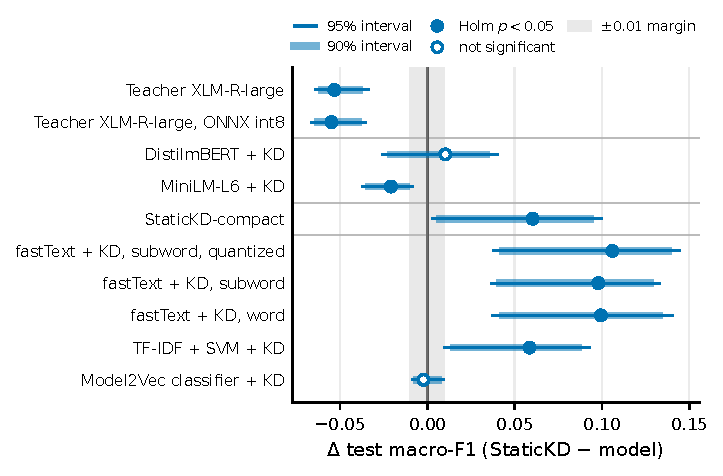
\includegraphics[width=\columnwidth]{figures/fig_sig_forest.pdf}
\caption{Selisih berpasangan macro-F1 \en{test} antara StaticKD dan tiap model lain (StaticKD dikurangi model). Garis tipis menunjukkan interval \en{site-cluster bootstrap} 95\%. Batang tebal menunjukkan interval 90\%. Penanda terisi berbeda signifikan setelah koreksi Holm. Pita berarsir adalah margin kesetaraan $\pm$0.01. Dua model fastText yang dilatih pada label GPT-4o berada di atas +0.4 dan tidak ditampilkan.}
\label{fig:sig-forest}
\end{figure}
Uji berpasangan pada Tabel~\ref{tab:sig} mengonfirmasi peringkat ini. Gambar~\ref{fig:sig-forest} memperlihatkan bahwa interval 95\% selisih StaticKD terhadap semua model ringan kecuali pengklasifikasi Model2Vec berada di atas nol sedangkan interval terhadap \en{teacher} dan MiniLM-L6 berada di bawah nol. $\Delta$macro-F1 StaticKD terhadap \en{teacher} adalah $-$0.053 [$-$0.065, $-$0.033] dan StaticKD mengungguli \en{teacher} hanya pada 7 dari 47 bahasa. MiniLM-L6 juga mempertahankan keunggulan yang signifikan atas StaticKD ($-$0.021 [$-$0.038, $-$0.008], $p=0.005$). StaticKD dan DistilmBERT tidak berbeda signifikan (+0.010, $p=1.000$) dan interval 90\% [$-$0.023, +0.036] dari selisih ini terlalu lebar untuk menunjukkan kesetaraan (TOST $p=0.428$). Uji Wilcoxon per bahasa juga tidak menemukan perbedaan yang konsisten antara kedua model ($p=0.604$ untuk macro-F1 dan 0.322 untuk akurasi). Uji McNemar mengunggulkan StaticKD atas DistilmBERT dalam akurasi ($p<0.001$) tetapi memperlakukan artikel dari situs yang sama sebagai independen.

Pengklasifikasi Model2Vec adalah satu-satunya model ringan yang menyamai StaticKD. $\Delta$macro-F1 antara kedua model adalah $-$0.002 [$-$0.009, +0.010] dengan interval 90\% sebesar [$-$0.008, +0.008] di dalam margin kesetaraan $\pm$0.01 (TOST $p=0.025$). Perbandingan per bahasa dengan pengklasifikasi Model2Vec juga tidak menunjukkan perbedaan yang konsisten pada kedua metrik (Wilcoxon $p=0.358$ untuk macro-F1 dan 0.534 untuk akurasi).

StaticKD unggul atas fastText + KD terkuantisasi sebesar +0.106 [+0.037, +0.145] dan atas TF-IDF + SVM sebesar +0.059 [+0.009, +0.093] ($p=0.040$). Macro-F1 StaticKD lebih tinggi daripada fastText + KD pada 40 dari 47 bahasa (Wilcoxon $p<0.001$). Keunggulan atas TF-IDF + SVM lebih sempit dengan macro-F1 StaticKD yang lebih tinggi pada 31 dari 47 bahasa (Wilcoxon $p=0.003$). Gambaran yang berbeda muncul dari akurasi per bahasa terhadap TF-IDF + SVM karena StaticKD lebih tinggi pada 24 bahasa dan lebih rendah pada 22 (Wilcoxon $p=0.127$).

Peringkat model hampir tidak berubah pada pemeriksaan terhadap struktur klaster \en{test set}. \en{Subset} dengan paling banyak lima artikel per situs dan pasangan bahasa--label menyisakan 8,139 artikel dengan skor 0.587 untuk StaticKD dan 0.627 untuk \en{teacher}. Hanya urutan StaticKD dan pengklasifikasi Model2Vec (0.583) yang berubah pada \en{subset} tersebut. Pembuangan sumber satu per satu menempatkan StaticKD di antara peringkat ketiga dan kelima dari sembilan model dan hanya pengklasifikasi Model2Vec serta DistilmBERT yang bertukar posisi dengannya. Setiap model fastText dan TF-IDF tetap paling sedikit 0.028 di bawah StaticKD.

Hasil uji berpasangan juga tidak berubah ketika kedua \en{transformer} membaca input yang lebih panjang. Pelatihan ulang dengan input 512 token menaikkan macro-F1 \en{test} MiniLM-L6 dan DistilmBERT menjadi 0.580 dan 0.547. MiniLM-L6 tetap unggul atas StaticKD ($-$0.035 [$-$0.049, $-$0.021], $p<0.001$) dan DistilmBERT tetap tidak berbeda signifikan dari StaticKD ($-$0.002 [$-$0.029, +0.022], $p=0.779$).

\subsection{Efisiensi CPU}
\label{sec:res-eff}
\begin{table*}[!t]
\caption{Efisiensi CPU pada P-Core yang Dipatok (Sampel dari \en{Test Set} Terpadu, 1c/4c = 1/4 \en{Core})}
\label{tab:eff}
\centering
\scriptsize
\resizebox{\textwidth}{!}{%
\begin{tabular}{@{}lcccccl@{}}
\toprule
Model & Latensi p50 / p95, 1c (ms) & Throughput 1c (dok/s) & Throughput 4c (dok/s) & RAM Model (MB) & Berkas (MB) & Dependensi \\
\midrule
Teacher XLM-R-large & 2,816 / 2,894 & 0.34 & 0.97 & 2,950 & 2,136 & torch, transformers \\
Teacher XLM-R-large, ONNX int8 & 1,190 / 1,229 & 0.79 & 2.53 & 1,375 & 537 & onnxruntime, transformers \\
DistilmBERT + KD & 193 / 202 & 5.05 & 15.6 & 1,059 & 516 & onnxruntime, transformers \\
MiniLM-L6 + KD & 56.5 / 61.9 & 16.9 & 48.8 & 1,235 & 408 & onnxruntime, transformers \\
\textbf{StaticKD} & 2.01 / 3.31 & 539 & 1,827 & 501 & 34 & numpy, tokenizers \\
StaticKD ringkas & 1.78 / 3.17 & 601 & 2,005 & 277 & 23 & numpy, tokenizers \\
fastText + KD, subword, terkuantisasi & 1.93 / 3.21 & 545 & 1,393 & 300 & 18 & fasttext, tokenizers \\
fastText + KD, subword & 2.07 / 3.62 & 489 & 1,184 & 1,122 & 839 & fasttext, tokenizers \\
TF-IDF + SVM + KD & 2.96 / 4.49 & 433 & 865 & 828 & 166 & scikit-learn, tokenizers \\
Pengklasifikasi Model2Vec + KD & 1.99 / 3.22 & 568 & 1,822 & 1,091 & 507 & model2vec, scikit-learn \\
\bottomrule
\end{tabular}}
\end{table*}
\begin{figure*}[!t]
\centering
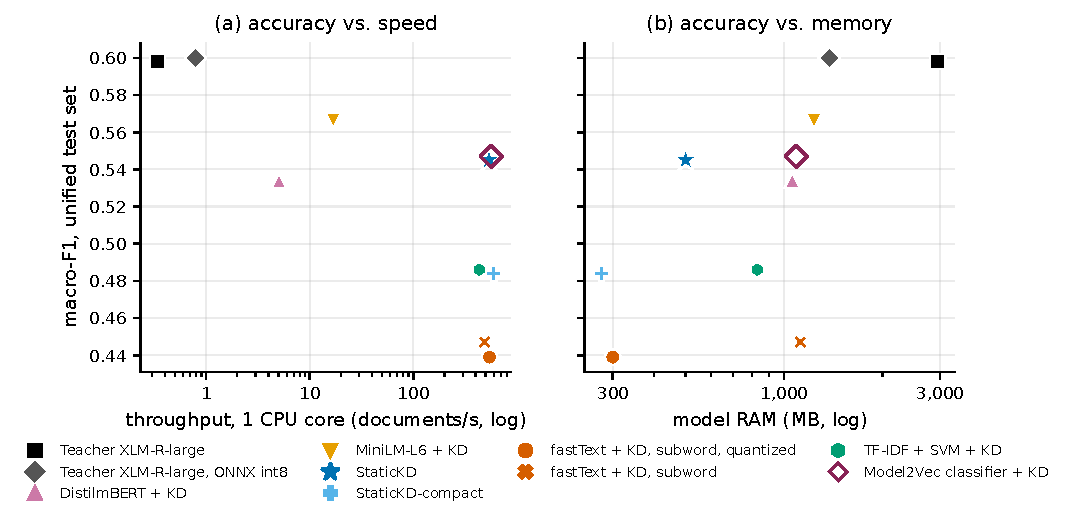
\includegraphics[width=0.85\textwidth]{figures/fig_tradeoff_memory.pdf}
\caption{Macro-F1 \en{test} pada \en{test set} terpadu terhadap (a) \en{throughput} CPU satu \en{core} dan (b) RAM model (skala log).}
\label{fig:tradeoff}
\end{figure*}
Tabel~\ref{tab:eff} menunjukkan bahwa \en{teacher} terlalu lambat di CPU untuk aliran artikel yang besar dan StaticKD menghilangkan biaya ini hampir seluruhnya. \en{Teacher} PyTorch fp32 memerlukan 2,816~ms per artikel pada satu \en{core} dan mencapai \en{throughput} 0.34 artikel per detik. Konfigurasi CPU terbaik untuk \en{teacher} adalah ONNX int8 (1,190~ms per artikel dan 0.79 artikel per detik). Kecepatan kedua konfigurasi ini berarti klasifikasi satu juta artikel per hari akan memerlukan 14.7 \en{core} (ONNX int8) hingga 33.7 \en{core} (PyTorch) untuk langkah ini saja. Beban yang sama memerlukan 0.02 \en{core} pada StaticKD.

Kecepatan StaticKD pada satu \en{core} melampaui semua model berbasis \en{transformer} dan mirip dengan model ringan lain. StaticKD memerlukan 2.01~ms per artikel dan dapat memproses 539 artikel per detik per \en{core} atau sekitar 682 kali kecepatan \en{teacher} ONNX int8 dan 1,572 kali kecepatan \en{teacher} PyTorch. MiniLM-L6 dan DistilmBERT hasil distilasi masih sekitar 32 dan 107 kali lebih lambat daripada StaticKD. Kecepatan satu \en{core} model ringan lain berkisar dari 433 artikel per detik untuk TF-IDF + SVM hingga 601 untuk varian ringkas. Tokenisasi membatasi kecepatan StaticKD karena memakan 98\% waktu prediksi satu \en{thread} dengan rata-rata 579 token per artikel sedangkan langkah merata-ratakan baris tabel yang menyusul tokenisasi mencapai 26,843 artikel per detik bila diukur sendiri.

StaticKD juga memerlukan berkas yang lebih kecil daripada \en{teacher} serta berkas dan RAM yang lebih kecil daripada pengklasifikasi Model2Vec. Berkas StaticKD 16 kali lebih kecil daripada berkas \en{teacher} ONNX int8. Pengklasifikasi Model2Vec yang menyamai akurasi StaticKD memerlukan 507~MB di \en{disk} dan 1,091~MB RAM dibandingkan dengan 501~MB RAM pada StaticKD. Gambar~\ref{fig:tradeoff} memperlihatkan bahwa StaticKD dan pengklasifikasi Model2Vec hampir berimpit pada panel (a) tetapi terpisah pada sumbu RAM di panel (b). RAM StaticKD tersebut sebagian besar diisi struktur \en{tokenizer} dan turun menjadi 277~MB pada varian ringkas. Model fastText + KD terkuantisasi lebih kecil (18~MB) dan memakai lebih sedikit RAM (300~MB) daripada StaticKD tetapi hanya mencapai macro-F1 \en{test} 0.439.

\subsection{Ablasi, \en{Temperature}, dan \en{Ensemble}}
\label{sec:res-abl}
\begin{table*}[!t]
\caption{Ablasi dan \en{Temperature} (Satu \en{Student}, Tanpa \en{Ensemble}). Rata-Rata $\pm$ Simpangan Baku atas \en{Seed}. $^{*}$ = Berbeda dari Resep Akhir (\en{Bootstrap} Berpasangan, Holm, $p<0.05$). $\Delta$ = Macro-F1 \en{Test} Dikurangi Macro-F1 \en{Test} Resep Akhir [95\% CI]. $^{\dagger}$ = Setara dalam $\pm$0.01 (TOST)}
\label{tab:ablation}
\centering
\scriptsize
\begin{tabular}{@{}lccccc@{}}
\toprule
Varian & Seed & Macro-F1 dev & Agreement held-out & Macro-F1 test & $\Delta$ macro-F1 test [95\% CI] \\
\midrule
\multicolumn{6}{@{}l}{\textit{Resep akhir}} \\
\quad Resep akhir (satu seed) & 10 & 0.755$\pm$0.010 & 0.808$\pm$0.001 & 0.542$\pm$0.004 & -- \\
\multicolumn{6}{@{}l}{\textit{Ablasi komponen}} \\
\quad Hard label teacher (cross-entropy) & 5 & 0.749$\pm$0.007 & 0.805$\pm$0.001 & 0.547$\pm$0.004 & +0.005 [$-$0.002, +0.010]$^{\dagger}$ \\
\quad EMMediaTopic saja (4 bahasa, 20k) & 5 & 0.723$\pm$0.006$^{*}$ & 0.730$\pm$0.001$^{*}$ & 0.491$\pm$0.002$^{*}$ & $-$0.051 [$-$0.064, $-$0.036] \\
\quad 130k dokumen (tanpa CC-News tambahan) & 5 & 0.736$\pm$0.009$^{*}$ & 0.799$\pm$0.002$^{*}$ & 0.541$\pm$0.002 & $-$0.002 [$-$0.008, +0.002]$^{\dagger}$ \\
\quad Embedding diinisialisasi acak & 5 & 0.715$\pm$0.005$^{*}$ & 0.739$\pm$0.004$^{*}$ & 0.422$\pm$0.006$^{*}$ & $-$0.120 [$-$0.166, $-$0.047] \\
\quad Embedding beku (hanya head linear) & 5 & 0.720$\pm$0.001$^{*}$ & 0.788$\pm$0.001$^{*}$ & 0.557$\pm$0.002 & +0.014 [$-$0.004, +0.024] \\
\quad Tanpa token dropout & 5 & 0.757$\pm$0.004 & 0.808$\pm$0.001 & 0.544$\pm$0.002 & +0.001 [$-$0.001, +0.003]$^{\dagger}$ \\
\quad Head MLP 512 unit (tidak dapat dilipat) & 5 & 0.762$\pm$0.009 & 0.813$\pm$0.002$^{*}$ & 0.551$\pm$0.006 & +0.009 [$-$0.000, +0.012] \\
\multicolumn{6}{@{}l}{\textit{Temperature}} \\
\quad $\tau=0.5$ & 5 & 0.750$\pm$0.004 & 0.807$\pm$0.002 & 0.546$\pm$0.005 & +0.004 [$-$0.002, +0.007]$^{\dagger}$ \\
\quad $\tau=2$ & 5 & 0.748$\pm$0.003 & 0.801$\pm$0.001$^{*}$ & 0.537$\pm$0.001 & $-$0.005 [$-$0.010, +0.008]$^{\dagger}$ \\
\quad $\tau=4$ & 5 & 0.723$\pm$0.004$^{*}$ & 0.791$\pm$0.001$^{*}$ & 0.529$\pm$0.002 & $-$0.014 [$-$0.020, +0.001] \\
\bottomrule
\end{tabular}
\end{table*}
\begin{table}[!t]
\caption{Macro-F1 Varian Terpilih menurut Jumlah Data Distilasi dalam Bahasa Artikel (\en{Test Set}, Rata-Rata atas \en{Seed})}
\label{tab:ablation-groups}
\centering
\footnotesize
\setlength{\tabcolsep}{3pt}
\resizebox{\columnwidth}{!}{%
\begin{tabular}{@{}lcccc@{}}
\toprule
Varian & Dev & Cukup ($\ge$500) & Sedikit ($<$500) & Tidak Ada (0) \\
\midrule
Resep akhir (satu seed) & 0.755 & 0.615 & 0.482 & 0.403 \\
Embedding beku (hanya head linear) & 0.720 & 0.607 & 0.541 & 0.440 \\
Embedding diinisialisasi acak & 0.715 & 0.567 & 0.182 & 0.161 \\
EMMediaTopic saja (4 bahasa, 20k) & 0.723 & 0.559 & 0.466 & 0.351 \\
Hard label teacher (cross-entropy) & 0.749 & 0.617 & 0.482 & 0.410 \\
Head MLP 512 unit (tidak dapat dilipat) & 0.762 & 0.613 & 0.484 & 0.421 \\
$\tau=2$ & 0.748 & 0.612 & 0.476 & 0.363 \\
\bottomrule
\end{tabular}}
\end{table}
\begin{figure}[!t]
\centering
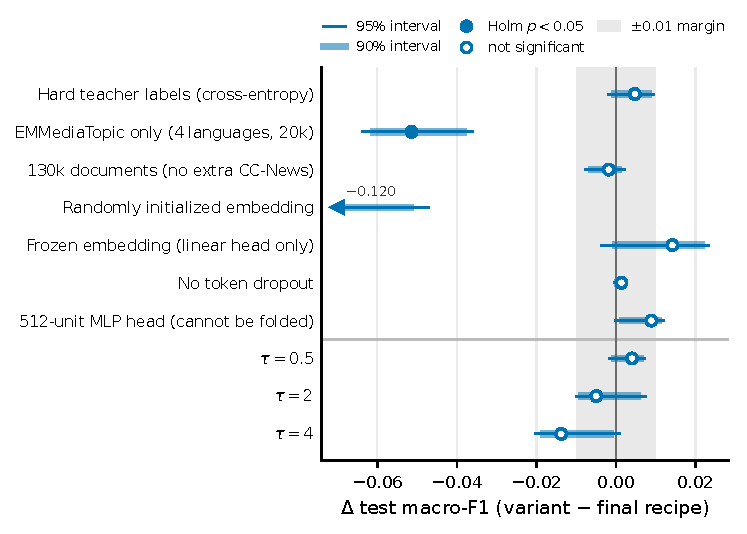
\includegraphics[width=\columnwidth]{figures/fig_ablation_forest.pdf}
\caption{Selisih macro-F1 \en{test} antara setiap varian ablasi dan resep akhir (varian dikurangi resep akhir). Pengodean mengikuti Gambar~\ref{fig:sig-forest}. Sebuah garis memisahkan ablasi komponen dari nilai \en{temperature}.}
\label{fig:abl-forest}
\end{figure}
Tabel~\ref{tab:ablation} menunjukkan bahwa sebagian besar akurasi berasal dari dua komponen: data distilasi multibahasa dan \en{embedding} hasil prapelatihan. \en{Student} yang didistilasi pada EMMediaTopic saja (4 bahasa) sebagai pengganti data distilasi multibahasa kehilangan 0.051 pada macro-F1 \en{test} dan 0.077 pada \en{agreement} \en{held-out}. Penggantian \en{embedding} potion hasil prapelatihan dengan inisialisasi acak menurunkan macro-F1 \en{test} lebih banyak daripada varian lain mana pun (0.120, $p<0.001$). Gambar~\ref{fig:abl-forest} memperlihatkan bahwa hanya kedua varian ini yang berbeda signifikan dari resep akhir pada macro-F1 \en{test}.

Pembekuan \en{embedding} membatasi pelatihan pada \en{head} linear di atas potion dan memberikan hasil yang tidak searah. Skor \en{development set} turun sebesar 0.035 ($p=0.040$) dan \en{agreement} \en{held-out} turun sebesar 0.020 ($p<0.001$). Macro-F1 \en{test} justru naik sebesar 0.014 dengan interval yang mencakup nol ([$-$0.004, +0.024], $p=1.000$). Tabel~\ref{tab:ablation-groups} menelusuri kenaikan ini ke bahasa dengan sedikit data distilasi (+0.059) dan ke bahasa tanpa data distilasi (+0.037). Bahasa dengan paling sedikit 500 dokumen menunjukkan arah sebaliknya dengan \en{embedding} beku yang sedikit lebih lemah pada kelompok ini ($-$0.007).

Tidak ada varian lain yang mengubah macro-F1 \en{test} secara signifikan. \en{Hard label} dari \en{teacher} menaikkan macro-F1 \en{test} sebesar 0.005 ($p=1.000$) dan menurunkan skor \en{development set} sebesar 0.006 ($p=1.000$). Interval 90\% dari selisih \en{test} berada di dalam margin kesetaraan ([$-$0.001, +0.009], TOST $p=0.017$). Uji ini menunjukkan bahwa \en{hard label} bekerja sebaik \en{soft label}. Pengurangan data menjadi 130 ribu dokumen menurunkan skor \en{test} sebesar 0.002 ($p=1.000$) dan \en{agreement} \en{held-out} sebesar 0.009 ($p<0.001$) tetapi selisih \en{test}-nya tetap lolos uji kesetaraan. Menghilangkan \en{token dropout} menaikkan macro-F1 \en{test} sebesar 0.001 ($p=1.000$) dan juga lolos uji kesetaraan. \en{Head} MLP yang tidak dapat dilipat menaikkan macro-F1 \en{test} sebesar 0.009 ($p=0.780$) tetapi tidak lolos uji kesetaraan karena interval 90\%-nya mencapai +0.012.

\en{Temperature} yang lebih tinggi tidak membantu. Pilihan umum $\tau=2$~\cite{hinton2015distilling} menurunkan \en{agreement} \en{held-out} sebesar 0.007 ($p<0.001$) dibandingkan dengan $\tau=1$. Macro-F1 \en{test} dan skor \en{development set} pada pilihan ini tidak berubah signifikan ($-$0.005 dan $-$0.006, keduanya $p=1.000$). Selisih \en{test} lolos uji kesetaraan pada $\tau=2$ maupun $\tau=0.5$. Nilai $\tau=4$ menurunkan skor \en{development set} dan \en{agreement} \en{held-out} secara signifikan serta skor \en{test} sebesar 0.014 yang tidak signifikan ($p=0.836$).

Memperbesar \en{ensemble} memberi kenaikan kecil. Tiga \en{seed} sebagai ganti satu \en{seed} menaikkan macro-F1 \en{test} dari 0.542 menjadi 0.544 dan \en{agreement} \en{held-out} dari 0.808 menjadi 0.810. Sepuluh \en{seed} menaikkan macro-F1 \en{test} menjadi 0.546. Kenaikan ini diperoleh tanpa biaya pada waktu inferensi karena \en{ensemble} berukuran berapa pun dilipat menjadi satu tabel.

\subsection{Analisis per Bahasa, Label, Sumber, dan Token}
\label{sec:res-lang}
Tabel~\ref{tab:groups} menunjukkan bahwa porsi skor \en{teacher} yang dipertahankan StaticKD lebih bervariasi menurut jumlah data distilasi dalam bahasa artikel daripada menurut asal label. Porsi per asal label berada antara 89.5\% untuk kategori penerbit dan 95.8\% untuk rubrik JSON-LD. Pengelompokan menurut data distilasi menunjukkan porsi yang turun dari 97.5\% pada bahasa dengan paling sedikit 500 dokumen distilasi menjadi 72.3\% pada bahasa tanpa data distilasi. Subkelompok tanpa data distilasi ini juga satu-satunya subkelompok di Tabel~\ref{tab:groups} tempat pengklasifikasi Model2Vec unggul atas StaticKD dengan selisih lebih dari 0.011 (0.429 berbanding 0.402).

\begin{table*}[!t]
\caption{Macro-F1 \en{Test} per Subkelompok. Kolom Terakhir: Macro-F1 StaticKD sebagai Persentase Macro-F1 \en{Teacher} pada Subkelompok yang Sama}
\label{tab:groups}
\centering
\scriptsize
\setlength{\tabcolsep}{3.5pt}
\begin{tabular}{@{}lrccccccccc@{}}
\toprule
Subkelompok & $n$ & Teacher & DistilmBERT & MiniLM & \textbf{StaticKD} & Model2Vec & fastText (q) & TF-IDF+SVM & fastText GPT & \% teacher \\
\midrule
\multicolumn{11}{@{}l}{\textit{Asal label}} \\
\quad anotasi manusia & 4,094 & 0.463 & 0.436 & 0.436 & 0.414 & 0.414 & 0.328 & 0.393 & 0.027 & 90\% \\
\quad kategori penerbit & 2,600 & 0.702 & 0.498 & 0.674 & 0.629 & 0.632 & 0.300 & 0.330 & 0.063 & 90\% \\
\quad rubrik JSON-LD & 6,050 & 0.651 & 0.629 & 0.634 & 0.624 & 0.618 & 0.582 & 0.609 & 0.136 & 96\% \\
\multicolumn{11}{@{}l}{\textit{Data distilasi bahasa}} \\
\quad cukup ($\ge$500) & 7,644 & 0.633 & 0.617 & 0.616 & 0.618 & 0.611 & 0.575 & 0.593 & 0.116 & 98\% \\
\quad sedikit ($<$500) & 2,243 & 0.537 & 0.344 & 0.496 & 0.478 & 0.475 & 0.195 & 0.227 & 0.037 & 89\% \\
\quad tidak ada (0) & 2,857 & 0.557 & 0.452 & 0.502 & 0.402 & 0.429 & 0.176 & 0.230 & 0.048 & 72\% \\
\multicolumn{11}{@{}l}{\textit{Wilayah}} \\
\quad Afrika & 3,044 & 0.697 & 0.532 & 0.576 & 0.542 & 0.550 & 0.325 & 0.408 & 0.085 & 78\% \\
\quad Asia Selatan & 2,681 & 0.575 & 0.410 & 0.544 & 0.509 & 0.510 & 0.241 & 0.276 & 0.046 & 88\% \\
\quad Asia Timur/Tenggara \& Timur Tengah & 1,574 & 0.636 & 0.620 & 0.621 & 0.622 & 0.612 & 0.555 & 0.629 & 0.085 & 98\% \\
\quad Eropa & 5,445 & 0.653 & 0.637 & 0.638 & 0.638 & 0.631 & 0.598 & 0.610 & 0.136 & 98\% \\
\multicolumn{11}{@{}l}{\textit{Cakupan prapelatihan teacher}} \\
\quad di luar prapelatihan XLM-R & 1,750 & 0.719 & 0.586 & 0.620 & 0.501 & 0.495 & 0.346 & 0.457 & 0.086 & 70\% \\
\quad dalam prapelatihan XLM-R & 10,994 & 0.609 & 0.549 & 0.585 & 0.576 & 0.572 & 0.471 & 0.503 & 0.096 & 95\% \\
\multicolumn{11}{@{}l}{\textit{Keragaman situs}} \\
\quad beragam ($\ge$10) & 5,225 & 0.657 & 0.642 & 0.643 & 0.642 & 0.637 & 0.601 & 0.616 & 0.134 & 98\% \\
\quad satu penerbit ($<$3) & 6,204 & 0.517 & 0.387 & 0.475 & 0.433 & 0.435 & 0.224 & 0.287 & 0.045 & 84\% \\
\quad sedang (3--10) & 1,315 & 0.559 & 0.556 & 0.539 & 0.543 & 0.532 & 0.503 & 0.533 & 0.089 & 97\% \\
\bottomrule
\end{tabular}
\end{table*}

Porsi ini juga berbeda menurut sumber artikel. MN-DS adalah satu-satunya sumber yang dianotasi langsung dengan topik IPTC dan StaticKD mempertahankan 97.4\% skor \en{teacher} pada sumber ini (0.535 berbanding 0.549). Porsi yang tinggi ini dicapai pada sumber tempat macro-F1 \en{teacher} sendiri lebih rendah daripada pada sumber lain mana pun. Porsi terkecil terdapat pada MasakhaNEWS (80.0\%) yang label manusianya mengikuti skema non-IPTC dan 11 dari 16 bahasanya tidak ada dalam data distilasi.

Panel kiri Gambar~\ref{fig:lang} menunjukkan bahwa selisih akurasi StaticKD terhadap \en{teacher} kecil pada bahasa yang tipikal dengan median $-$0.024 per bahasa. Selisih ini menyempit seiring bertambahnya jumlah data distilasi ($\rho=0.52$, $p<0.001$). \en{Agreement} \en{held-out} StaticKD dengan \en{teacher} naik seiring tingkat keyakinan \en{teacher} ($\rho=0.71$, $p<0.001$) tetapi hubungannya dengan log jumlah data distilasi ($\rho=0.31$) tidak signifikan setelah koreksi Holm ($p=0.067$). \en{Agreement} juga tidak berbeda signifikan antaraksara (Kruskal--Wallis $H=10.37$, $p=0.067$). Panel kanan Gambar~\ref{fig:lang} memperlihatkan bahwa \en{agreement} \en{held-out} StaticKD lebih tinggi daripada \en{agreement} fastText + KD terkuantisasi pada 52 dari 53 bahasa.

Titik lemah StaticKD adalah sekelompok bahasa Afrika. StaticKD hanya mencapai rata-rata akurasi 0.407 pada bahasa yang berada di luar prapelatihan XLM-R dan juga tidak ada dalam data distilasi (Igbo, Luganda, Lingala, Pidgin Nigeria, Kirundi, Shona, Tigrinya, dan Yoruba). \en{Teacher} mencapai 0.643 pada bahasa yang sama. StaticKD lebih akurat pada bahasa India yang tidak atau hampir tidak ada dalam data distilasi daripada pada bahasa Afrika tersebut.

Empat bahasa India (Bangla, Malayalam, Odia, dan Punjabi) menunjukkan perilaku StaticKD pada teks yang token-tokennya hampir tidak pernah muncul dalam pelatihan. StaticKD mencapai 0.748 pada berita Bangla meskipun bahasa ini tidak ada dalam data distilasi. Baik fastText + KD maupun TF-IDF + SVM anjlok pada artikel yang sama (0.191 dan 0.010). Paling sedikit 67\% kemunculan token dalam bahasa-bahasa ini berasal dari token yang muncul kurang dari 10 kali dalam data distilasi. StaticKD masih mencapai rata-rata akurasi 0.624 pada bahasa tersebut dibandingkan dengan 0.738 untuk \en{teacher}. Varian ringkas menghapus token langka ini dari \en{tokenizer} dan akurasinya pada keempat bahasa ini turun menjadi 0.013. Akurasi kedua model pada bahasa lainnya adalah 0.578 untuk varian ringkas dan 0.640 untuk StaticKD penuh.

\begin{figure*}[!t]
\centering
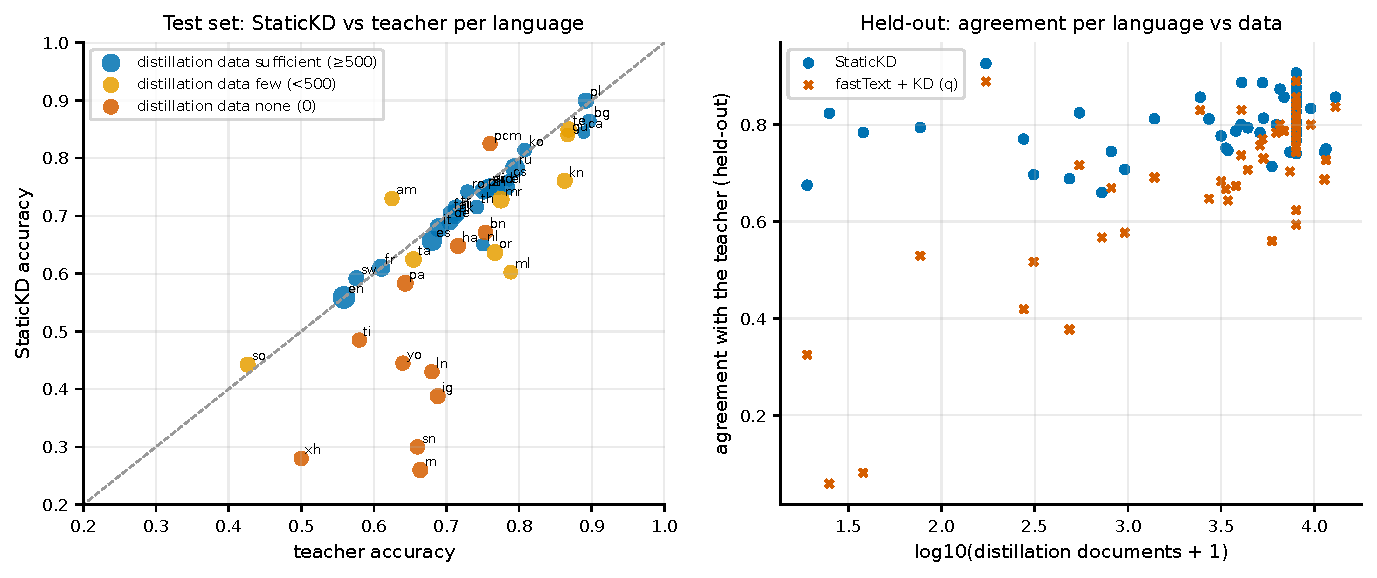
\includegraphics[width=0.8\textwidth]{figures/fig_per_language.pdf}
\caption{Kiri: akurasi StaticKD terhadap akurasi \en{teacher} per bahasa \en{test} (warna menunjukkan data distilasi bahasa, ukuran menunjukkan jumlah artikel). Kanan: \en{agreement} \en{held-out} per bahasa terhadap jumlah data distilasi untuk StaticKD dan fastText + KD terkuantisasi.}
\label{fig:lang}
\end{figure*}

Kinerja StaticKD berbeda antarlabel dan empat label tersulitnya juga termasuk label tersulit bagi \en{teacher}. Skor StaticKD pada keempat label ini adalah \emph{society} (0.16), \emph{disaster} (0.29), \emph{human interest} (0.32), dan \emph{conflict} (0.37). Kekeliruan yang paling sering adalah prediksi \emph{human interest} untuk \emph{society}, \emph{arts} untuk \emph{human interest}, dan \emph{politics} untuk \emph{society} dengan porsi masing-masing 20\%. StaticKD paling baik pada \emph{sport} (0.88), \emph{weather} (0.84), dan \emph{education} (0.75). Selisih terbesar terhadap \en{teacher} terjadi pada \emph{environment} ($-$0.17), \emph{religion} ($-$0.15), dan \emph{arts} ($-$0.08).

Tabel token StaticKD juga menunjukkan token mana yang membawa sinyal topik artikel. Menyisakan hanya 10\% token paling spesifik pada setiap artikel membuat macro-F1 \en{test} hampir tidak berubah (0.543 dengan sekitar 58 token per artikel berbanding 0.545 dengan semua token). Pilihan acak 10\% token hanya menghasilkan 0.435.

\subsection{Kalibrasi dan Mode \en{Cascade}}
\begin{table}[!t]
\caption{\en{Cascade} StaticKD $\rightarrow$ \en{Teacher} ONNX Int8 pada \en{Test Set} (\en{Throughput} Efektif Satu \en{Core})}
\label{tab:cascade}
\centering
\footnotesize
\setlength{\tabcolsep}{2.5pt}
\resizebox{\columnwidth}{!}{%
\begin{tabular}{@{}lccccc@{}}
\toprule
$\theta$ & Porsi StaticKD & Akurasi pada porsi & Macro-F1 & Akurasi & dok/s \\
\midrule
0 (StaticKD saja) & 100.0\% & 0.641 & 0.545 & 0.641 & 539 \\
0.5 & 80.8\% & 0.732 & 0.586 & 0.690 & 4.09 \\
0.6 & 74.0\% & 0.760 & 0.593 & 0.697 & 3.02 \\
0.7 & 67.4\% & 0.788 & 0.600 & 0.702 & 2.41 \\
0.8 & 60.3\% & 0.813 & 0.602 & 0.703 & 1.98 \\
0.9 & 51.7\% & 0.839 & 0.602 & 0.703 & 1.63 \\
Teacher saja & 0.0\% & -- & 0.600 & 0.699 & 0.79 \\
\bottomrule
\end{tabular}}
\end{table}
Tingkat keyakinan StaticKD lebih terkalibrasi daripada tingkat keyakinan \en{teacher}. ECE StaticKD adalah 0.041 pada \en{development set} dan 0.139 pada \en{test set} berbanding 0.090 dan 0.245 untuk \en{teacher}. Kedua model menjadi terlalu yakin pada \en{test set} di luar distribusi. Mode \en{cascade} memakai tingkat keyakinan ini untuk menentukan artikel yang diputuskan StaticKD. Tabel~\ref{tab:cascade} menunjukkan bahwa ambang $\theta$ yang lebih tinggi menyerahkan lebih banyak artikel kepada \en{teacher}. Akurasi pada porsi StaticKD karena itu naik dari 0.732 menjadi 0.839 tetapi \en{throughput} efektif turun dari 4.09 menjadi 1.63 artikel per detik. Mode \en{cascade} pada $\theta=0.8$ mencapai akurasi keseluruhan 0.703 dan macro-F1 0.602 berbanding 0.699 dan 0.600 untuk \en{teacher} saja. StaticKD sendiri memutuskan 60.3\% artikel dalam \en{cascade} ini dengan akurasi 0.813. \en{Throughput} efektif \en{cascade} ini adalah 1.98 artikel per detik per \en{core} atau 2.5 kali \en{throughput} \en{teacher} (0.79).

\section{Pembahasan}
\label{sec:discussion}
\subsection{Informasi yang Dipertahankan Tabel Token}
\en{Lookup} tabel mempertahankan sekitar sembilan per sepuluh macro-F1 \en{teacher} dan memangkas waktu inferensi sekitar tiga orde besaran (Bagian~\ref{sec:res-acc} dan~\ref{sec:res-eff}). Sebuah tabel sudah cukup karena sebagian kecil token yang spesifik untuk topik membawa hampir seluruh sinyal topik dalam artikel (Bagian~\ref{sec:res-lang}). Temuan ini sesuai dengan pengamatan~\cite{galke2022bow} bahwa representasi tanpa urutan sudah kompetitif untuk klasifikasi topik.

Skor StaticKD terendah terjadi pada \emph{society}, \emph{disaster}, \emph{human interest}, dan \emph{conflict} tetapi skor rendah ini tidak khas bagi \en{student}. Label yang sama termasuk label tersulit bagi \en{teacher} (Bagian~\ref{sec:res-lang}) dan \emph{society} serta \emph{human interest} sulit bahkan bagi anotator manusia~\cite{kuzman2025llm}. Selisih yang tersisa terhadap \en{teacher} terletak pada label lain dan pada bahasa yang kurang terwakili dalam data distilasi (Bagian~\ref{sec:res-lang}).

\subsection{Sumber Akurasi}
Kontribusi terbesar berasal dari inisialisasi multibahasa hasil prapelatihan dan kontribusi terbesar kedua dari data distilasi multibahasa yang dilabeli \en{teacher}. Inisialisasi acak mengurangi macro-F1 \en{test} sebesar 0.120 berbanding 0.051 untuk penghapusan data multibahasa. Bukti paling langsung tentang peran inisialisasi berasal dari varian ringkas pada empat bahasa India yang hampir tidak muncul dalam data distilasi (Bagian~\ref{sec:res-lang}). \en{Embedding} token langka dalam bahasa-bahasa ini tetap dekat dengan nilai potion karena pelatihan jarang atau tidak pernah memperbaruinya. Akurasi StaticKD dalam bahasa-bahasa ini masih mendekati akurasinya pada bahasa lain tetapi turun hampir ke nol setelah \en{tokenizer} ringkas menghapus token-token ini. Penurunan ini mengungkap bahwa transfer ke bahasa tanpa data bergantung pada \en{embedding} yang hampir tidak diubah pelatihan. \en{Head} linear yang dipelajari dari bahasa kaya data tetap berlaku untuk \en{embedding} tersebut karena \en{embedding} ini berada dalam ruang yang sama dengan \en{embedding} yang telah dilatih. Peran inisialisasi ini juga membedakan StaticKD dari Sparse Distillation~\cite{ye2022sparse} yang melatih tabel n-gram dari awal. \en{Embedding} multibahasa hasil prapelatihan yang dilipat menjadi 17 logit per token memungkinkan transfer ke bahasa yang tidak ada dalam data distilasi.

Pembekuan \en{embedding} menaikkan rata-rata skor bahasa dengan data distilasi yang sedikit atau tidak ada (Tabel~\ref{tab:ablation-groups}). \en{Fine-tuning} menggeser \en{embedding} token milik bahasa pelatihan sedangkan token dari bahasa lain tetap berada pada posisi yang diberikan oleh potion. \en{Head} model telah menyesuaikan diri dengan \en{embedding} yang bergeser dan kurang cocok dengan token yang tidak bergeser. Pergeseran yang sama membuat model lebih cocok dengan bahasa pelatihan sehingga \en{embedding} beku memberikan skor \en{development set} yang lebih rendah. \en{Fine-tuning} dan pembekuan karena itu mungkin mempertukarkan kecocokan dengan bahasa pelatihan dan penyelarasan lintas bahasa yang diwarisi dari potion. \en{Development set} dalam bahasa pelatihan hanya mengukur sisi pertama pertukaran ini sehingga resep akhir yang dipilih pada set tersebut memakai \en{fine-tuning}. Pembekuan tidak memberikan kenaikan signifikan pada seluruh \en{test set} tetapi layak diuji untuk penerapan yang menyasar bahasa tanpa data distilasi.

Perbandingan MiniLM-L6 dan DistilmBERT sebagai dua \en{student} \en{transformer} juga menunjuk pada peran representasi multibahasa awal. Kedua model ini belajar dari data distilasi yang sama dan sama-sama memiliki enam lapisan tetapi representasi awal keduanya berbeda karena MiniLM berasal dari distilasi XLM-R-large dan DistilmBERT dari mBERT. Hanya MiniLM-L6 yang menutup sebagian selisih terhadap \en{teacher} (Tabel~\ref{tab:sig}).

Akurasi StaticKD dan pengklasifikasi Model2Vec kemungkinan terutama berasal dari \en{embedding} yang dipakai bersama dan data yang dilabeli \en{teacher} alih-alih dari \en{head}. Pengklasifikasi Model2Vec memakai \en{embedding} dan data yang sama dengan StaticKD tetapi belajar dari label teratas \en{teacher} dan menambahkan bobot per token serta lapisan tersembunyi (Tabel~\ref{tab:baselines}). Model ini tetap mencapai macro-F1 \en{test} yang sama dengan StaticKD dalam margin kesetaraan $\pm$0.01. Margin ini kurang dari separuh selisih antara StaticKD dan MiniLM-L6 (Tabel~\ref{tab:sig}). Ablasi di Bagian~\ref{sec:res-abl} juga tidak menunjukkan kenaikan signifikan pada macro-F1 \en{test} dari \en{head} MLP.

\en{Soft label} menambah sedikit atau tidak menambah apa pun. \en{Hard label} \en{teacher} setara dengan \en{soft label} pada $\tau=1$ dalam $\pm$0.01 macro-F1 dan \en{temperature} yang lebih tinggi tidak pernah mengungguli $\tau=1$ (Bagian~\ref{sec:res-abl}). Pola ini sesuai dengan literatur tentang kesenjangan kapasitas~\cite{zhang2025law,wang2026rckd}. Satu lapisan linear di atas \en{embedding} yang dirata-ratakan mungkin tidak mampu merepresentasikan struktur antarkelas pada ekor distribusi \en{teacher} (\en{dark knowledge})~\cite{zhao2022dkd}. Nilai $\tau$ yang tinggi menuntut \en{student} meniru bentuk distribusi di luar kapasitasnya.

\en{Agreement} dengan \en{teacher} juga tidak selalu memprediksi akurasi pada label independen sehingga tidak cukup untuk memilih \en{student}~\cite{stanton2021kd}. Pemangkasan data menjadi 130 ribu dokumen menurunkan \en{agreement} secara signifikan tetapi membiarkan macro-F1 \en{test} tetap setara dengan resep akhir. Varian \en{embedding} beku memperoleh \en{agreement} \en{held-out} yang lebih rendah tetapi macro-F1 \en{test} yang lebih tinggi meskipun kenaikan ini tidak signifikan (Bagian~\ref{sec:res-abl}). Pemilihan \en{student} karena itu sebaiknya memakai label yang tidak berasal dari \en{teacher} dan \en{development set} di luar distribusi pelatihan.

\subsection{Bahasa yang Lemah}
Kinerja per bahasa naik seiring seberapa baik suatu bahasa terwakili dalam data distilasi dan data prapelatihan. Kelompok terlemah terdiri atas bahasa Afrika di luar prapelatihan XLM-R yang juga tidak ada dalam data distilasi (Bagian~\ref{sec:res-lang}). \en{Subword} yang dipakai bersama dengan bahasa lain dan konteks kalimat mungkin menjelaskan mengapa \en{teacher} tetap lebih akurat daripada StaticKD pada bahasa-bahasa ini. Perbaikan termurah tidak memerlukan perubahan arsitektur karena \en{teacher} dapat melabeli berita dalam bahasa-bahasa ini untuk ditambahkan ke data distilasi. Ablasi data dan korelasi antara selisih akurasi dan jumlah data ($\rho=0.52$) mendukung penambahan berita semacam ini.

\subsection{Implikasi Praktis}
StaticKD cocok untuk \en{pipeline} \en{real-time} pada server tanpa GPU dan dapat disesuaikan bila pekerjaan menuntut akurasi lebih tinggi atau RAM lebih kecil. Pengklasifikasi Model2Vec dan StaticKD berjalan dengan kecepatan serupa tetapi StaticKD dilipat menjadi satu tabel sehingga berkas dan RAM-nya lebih kecil dan model ini hanya memerlukan pustaka \texttt{numpy} dan \texttt{tokenizers} (Tabel~\ref{tab:eff}). Probabilitas keluaran StaticKD lebih terkalibrasi daripada probabilitas \en{teacher} sehingga memungkinkan mode \en{cascade} yang cocok untuk pekerjaan \en{batch} yang memerlukan akurasi setingkat \en{teacher}. Varian ringkas StaticKD menurunkan RAM tetapi hanya disarankan bila semua bahasa sasaran sudah tercakup dalam data distilasi.

\subsection{Keterbatasan}
\label{sec:limitations}
Skor \en{test} seharusnya dibaca dengan memperhatikan sifat label. Artikel tentang kasus kriminal yang melibatkan seorang atlet dapat secara sah berada di rubrik olahraga sedangkan sebuah model dapat melabeli artikel yang sama sebagai \emph{crime}. Kedua jawaban masuk akal karena IPTC memungkinkan beberapa topik per artikel. Perbandingan antarmodel tetap adil karena semua model dinilai terhadap label yang sama. Cakupan studi ini terbatas pada klasifikasi label tunggal pada label IPTC tingkat atas sehingga artikel multitopik dan label pada tingkat yang lebih dalam belum diuji.

Label rubrik dan kategori penerbit mengikuti cara penerbit mengategorikan artikel sehingga skor absolut pada label ini mengukur kesesuaian dengan cara tersebut. Konvensi rubrik berbeda dari satu penerbit ke penerbit lain dan sebuah rubrik mencerminkan satu pandangan editorial atas artikel yang mungkin mencakup beberapa topik. Keterbatasan label editorial ini terutama berlaku untuk \emph{society}, \emph{human interest}, \emph{lifestyle}, dan label lain dengan batas yang tidak jelas.

Sebagian besar label \en{test set} tidak dianotasi langsung dengan topik IPTC sehingga validitasnya bergantung pada pemetaan. Anotasi langsung dengan topik IPTC hanya ada di MN-DS dan hanya mencakup bahasa Inggris sedangkan \en{test set} IPTC multibahasa dari Kuzman dan Ljube\v{s}i\'c~\cite{kuzman2025llm} tidak tersedia untuk publik. Label MasakhaNEWS juga berasal dari anotator manusia tetapi mengikuti skema non-IPTC dan kemudian dipetakan ke IPTC. Label rubrik dipetakan dengan tabel yang disusun secara konservatif dan divalidasi terhadap pohon IPTC sebelum dievaluasi dan dikoreksi secara manual tetapi evaluasi manual ini tidak menghasilkan ukuran kesepakatan antarpeninjau.

Cakupan label tidak merata antarbahasa. Median jumlah label yang muncul dalam setiap bahasa adalah 7 dan bahasa-bahasa Afrika hanya mencakup tiga sampai lima topik umum. Skor per bahasa tidak dapat dibandingkan secara langsung antara bahasa dengan cakupan label yang berbeda karena macro-F1 dihitung atas label yang ada.

Keragaman situs juga terbatas. Dua puluh tujuh bahasa memiliki kurang dari 3 situs efektif. Artikel dalam bahasa tersebut sebagian besar berasal dari MasakhaNEWS, L3Cube-IndicNews, \en{dataset} berita Bangla, atau satu atau dua situs CC-NEWS. Klaim tentang bahasa-bahasa ini hanya berlaku untuk sumber-sumber tersebut. \en{Site-cluster bootstrap} melebarkan interval kepercayaan bahasa-bahasa ini secara sepadan. Semua interval \en{test set} bertumpu pada sejumlah kecil sumber independen karena seluruh \en{test set} hanya memiliki jumlah efektif 13.8 klaster.

Pilihan pembanding, anggaran penyetelan, dan panjang input \en{transformer} membatasi perbandingan StaticKD dengan model lain. Sparse Distillation~\cite{ye2022sparse} tidak dijalankan sebagai \en{baseline}. Metode ini berbeda dari fastText + KD dan dari ablasi inisialisasi acak dalam lapisan tersembunyi \en{deep averaging network}-nya, target \en{soft-logit}-nya, dan tabel n-gram berskala miliar parameter yang dirancang untuk bahasa Inggris. Anggaran penyetelan tidak sama untuk semua model. Resep StaticKD ditetapkan pada \en{development set} sebelum \en{test set} dibangun dan \en{baseline} fastText serta TF-IDF disetel pada set yang sama dengan \en{grid} kecil. Pengklasifikasi Model2Vec memakai pengaturan bawaan pustaka dan model \en{transformer} mengikuti resep \en{fine-tuning} standar yang hanya mencari $\tau$ untuk MiniLM-L6. MiniLM-L6 dan DistilmBERT juga membaca paling banyak 256 token dalam perbandingan utama sehingga kedua model hanya mendapat kurang dari separuh teks sebagian besar artikel \en{test}. Pelatihan ulang kedua model dengan 512 token menaikkan macro-F1 \en{test} sebesar 0.014 dan 0.012 tanpa mengubah hasil perbandingan dengan StaticKD (Bagian~\ref{sec:res-acc}).

Pengukuran efisiensi bergantung pada satu mesin. Seluruh \en{benchmark} dijalankan pada satu laptop (Bagian~\ref{sec:effprotocol}) dan latensi \en{teacher} serta model \en{transformer} hanya diukur pada 100 dokumen. Angka absolut akan berbeda pada server tetapi rasio antarmodel yang diukur dengan protokol yang sama tetap informatif.

Kelemahan StaticKD pada bahasa Afrika yang tidak ada dalam data distilasi maupun data prapelatihan (Bagian~\ref{sec:res-lang}) berarti filter topik yang berbasis model ini dapat lebih sering salah mengklasifikasikan atau membuang berita dalam bahasa-bahasa ini. Akurasi seharusnya dipantau per bahasa selama penerapan. Artikel dengan tingkat keyakinan rendah seharusnya diarahkan ke \en{teacher} melalui mode \en{cascade}.

\en{Teacher} membatasi kinerja \en{student} dari atas dan mewariskan kesalahan serta biasnya kepada \en{student}. Kesalahan warisan ini tidak terlihat pada \en{held-out set} karena set ini mengukur \en{agreement} dengan \en{teacher} dan bukan kebenaran.

\section{Kesimpulan}
\label{sec:conclusion}
Pengklasifikasi IPTC multibahasa terbuka memerlukan 1.2 hingga 2.8 detik per artikel pada satu \en{core} CPU. StaticKD mendistilasi pengklasifikasi ini menjadi tabel berisi 17 logit per token. \en{Student} yang menghasilkan tabel ini diinisialisasi dari \en{embedding} statis multibahasa dan kemudian dilatih pada 285,999 artikel berlabel \en{teacher} dalam 69 bahasa. Evaluasi memakai 12,744 artikel \en{test} dalam 47 bahasa yang labelnya tidak berasal dari \en{teacher}. \en{Test set} ini dapat dipakai ulang untuk mengevaluasi pengklasifikasi IPTC lain.

StaticKD mencapai macro-F1 0.545 pada \en{test set} tersebut (91.1\% dari skor \en{teacher}) dan memproses 539 artikel per detik per \en{core} CPU. Kecepatan ini sekitar 682 kali kecepatan \en{teacher} ONNX int8. Model berukuran 34~MB ini juga tidak memerlukan pustaka \en{deep learning}. Pengklasifikasi Model2Vec yang dilatih pada label \en{teacher} yang sama setara dengan StaticKD pada macro-F1 \en{test} tetapi memiliki berkas 15 kali lebih besar dan memerlukan memori dua kali lipat.

Ablasi menunjukkan bahwa akurasi \en{student} kecil ini terutama berasal dari data distilasi multibahasa dan \en{embedding} multibahasa hasil prapelatihan sedangkan \en{soft label} tidak lebih baik daripada \en{hard label}. \en{Embedding} beku menurunkan skor \en{development set} tetapi memberikan rata-rata skor yang lebih tinggi pada bahasa dengan data distilasi yang sedikit atau tidak ada meskipun kenaikan pada seluruh \en{test set} tidak signifikan.

StaticKD paling lemah pada label \emph{society}, \emph{disaster}, \emph{human interest}, dan \emph{conflict} serta pada bahasa yang tidak muncul dalam data distilasi maupun data prapelatihan \en{teacher}. Kelemahan pada bahasa ini menuntut perluasan data distilasi ke bahasa yang lemah dan terutama ke bahasa Afrika di luar prapelatihan XLM-R. \en{Fine-tuning} juga dapat memakai \en{regularizer} yang menjaga \en{embedding} tetap dekat dengan ruang hasil prapelatihan. \en{Regularizer} semacam ini mungkin memberikan akurasi dalam distribusi dan transfer lintas bahasa sekaligus.

Penelitian berikutnya juga dapat menekan biaya StaticKD dan memperluas tugas serta evaluasinya. \en{Tokenizer} yang lebih cepat seperti \en{lookup} langsung dari kata ke tabel menjadi sumber kecepatan berikutnya karena tokenisasi memakan 98\% waktu inferensi StaticKD. Pemangkasan kosakata untuk memperkecil model harus mempertahankan token langka yang menjadi sandaran bahasa dengan data distilasi yang sedikit atau tidak ada. Masalah lain yang masih terbuka adalah \en{head} nonlinear murah dengan \en{embedding} terkuantisasi, klasifikasi hierarkis hingga IPTC tingkat 2, klasifikasi multilabel, dan anotasi IPTC oleh manusia pada sampel multibahasa dari \en{test set}.

\section*{Ketersediaan Kode, Model, dan Data}
Kode untuk studi ini tersedia di \todo{URL GitHub dan DOI Zenodo} dan mencakup pengumpulan data, penyusunan \en{test set}, pelabelan oleh \en{teacher}, pelatihan, evaluasi, dan \en{benchmarking}. Lokasi yang sama menyediakan \en{notebook} yang mereproduksi setiap angka, tabel, dan gambar dalam makalah ini. Tabel pemetaan rubrik ke IPTC juga dirilis bersama kode. Model StaticKD tersedia di \todo{URL Hugging Face}. \en{Test set} dirilis bersama skrip rekonstruksinya sebagai manifes berisi URL atau ID artikel, label, asal label, dan \en{hash} teks. Teks artikel tidak didistribusikan ulang karena hak cipta penerbit dan lisensi \en{dataset} sumber. EMMediaTopic tersedia dari repositori CLARIN.SI~\cite{emmediatopic2025}. Lisensi aset yang dipakai dan dirilis dalam studi ini dicantumkan bersama kode.

\section*{Ucapan Terima Kasih}
Para penulis berterima kasih kepada Departemen Teknik Informatika, Institut Teknologi Sepuluh Nopember, atas dukungannya terhadap penelitian ini. Para penulis memakai Claude Opus 5.5 (Anthropic) di bawah arahan mereka untuk menjajaki pilihan desain metode dan untuk menjalankan eksperimen eksploratif dan eksperimen akhir. Model ini juga menulis kode eksperimen, mengolah data (termasuk draf pertama tabel pemetaan rubrik ke IPTC), dan menyusun draf sebagian teks naskah. Para penulis menulis dan merevisi naskah sendiri, meninjau dan memverifikasi semua kode, data, dan hasil, serta bertanggung jawab penuh atas isi dan klaim naskah.

\bibliographystyle{IEEEtran}
\bibliography{../paper_final/references}

\begin{IEEEbiographynophoto}{Obi Kastanya}
\todo{biografi penulis}
\end{IEEEbiographynophoto}

\begin{IEEEbiographynophoto}{Ananta Dwi Prayoga Alwy}
\todo{biografi penulis}\EOD
\end{IEEEbiographynophoto}

\end{document}
